\documentclass{itkmitlcoop}

\usepackage{afterpage}
\usepackage{graphicx,amsmath,latexsym,amssymb,amsthm}
\usepackage{indentfirst}
\usepackage{cite}
\usepackage{float}
\usepackage{wrapfig}
\usepackage{eso-pic} 
\usepackage[labelfont=bf]{caption}
\graphicspath{ {images/} }

\makeatletter
% \patchcmd{<cmd>}{<search>}{<replace>}{<succes>}{<failure>}
\patchcmd{\@chapter}{\addtocontents{lof}{\protect\addvspace{10\p@}}}{}{}{}% LoF
\patchcmd{\@chapter}{\addtocontents{lot}{\protect\addvspace{10\p@}}}{}{}{}% LoT
\makeatother

% Your thesis title (THAI)
\newcommand{\ThesisTiTle}{ระบบจัดการโฆษณาแบบจำกัดจำนวนการคลิกและการแสดงโฆษณา}
% Your thesis title (ENG)
\newcommand{\ThesisTiTleENG}{ADVERTISEMENT MANAGEMENT SYSTEM BASED ON LIMITED NUMBER OF CLICKS AND IMPRESSIONS}
\newcommand{\ThesisTiTleENGSnakecase}{Advertisement Management System Based on Limited Number of Clicks and Impressions}
% Your name
\newcommand{\AuName}{มาวิน จงไกรรัตนกุล}
% Your name ENG
\newcommand{\AuNameENG}{MAWIN JONGKRIRATTANAKUL}
\newcommand{\AuNameENGSnakecase}{Mawin Jongkrirattanakul}
% Department / Program
\newcommand{\DepartmentENG}{Information Technology}
% Your student ID
\newcommand{\SId}{59070141}
% Your advisor
\newcommand{\Advisor}{รองศาสตราจารย์ ดร.กิติ์สุชาต  พสุภา}
% Your advisor
\newcommand{\AdvisorENG}{Associate Professor Dr. Kitsuchart Pasupa}
% Your advisor employee
\newcommand{\Exami}{คุณ ธนพล เนรัญชร}
% ชื่อสถานประกอบการ
\newcommand{\Company}{บริษัท วงใน มีเดีย จำกัด (สำนักงานใหญ่)}
% ภาคเรียนที่ (in normal letters)
\newcommand{\Sem}{1}
% ปีการศึกษา (in normal letters)
\newcommand{\AcaY}{2562}
% ปีการศึกษา (in normal letters)
\newcommand{\AcaYAD}{2019}
% วันส่งรายงาน
\newcommand{\SubD}{2 ธันวาคม พ.ศ. 2562}
% วันเริ่มทำงาน
\newcommand{\StartDWork}{4 มิถุนายน พ.ศ. 2562}
% วันสุดท้ายของการทำงาน
\newcommand{\EndDWork}{29 พฤศจิกายน พ.ศ. 2562}
% ที่อยู่สถานประกอบการ
\newcommand{\Address}{เลขที่ 8 ถนนสุขุมวิท แขวงพระโขนง เขตคลองเตย จังหวัดกรุงเทพมหานคร \\ รหัสไปรษณีย์ 10110 โทรศัพท์ 0-2821-5788}
% เว็บไซต์สถานประกอบการ
\newcommand{\Website}{https://www.wongnai.com}
% ตำแหน่งานที่ปฏิบัติ
\newcommand{\Position}{Software Engineer (Backend)}

\begin{document}    
    \frontmatter
    \lhead{}\rhead{}\chead{}\lfoot{}\cfoot{\thepage}\rfoot{}
    \makecover    
    \makeinnercover
    \makeengcover
    \makecopyrightcover
    \makeletter
    \makeack{
        \begin{enumerate}
            \item คุณ ธนพล เนรัญชร \quad \quad ตำแหน่ง Technical Director (พนักงานที่ปรึกษา)
            \item คุณ ปาลิตา เตชะนิเวศน์ \quad ตำแหน่ง Software Engineer (Backend) 
        \end{enumerate}
    }
    \makeapproveletter
   
    % Setting margin for page numbering on frontmatter
    \newgeometry{top=1in, bottom=1in, left=1.5in, right=1in, includefoot}
    
    \makeabstract{
    	รายงานการปฏิบัติงานสหกิจศึกษาฉบับนี้กล่าวถึงที่มาและความสำคัญ, รายละเอียด, การออกแบบ และกระบวนการทำงานของระบบจัดการโฆษณาแบบจำกัดจำนวนการคลิกและการแสดงโฆษณา รวมไปถึงลักษณะขั้นตอนการทำงานเพื่อให้ได้มาซึ่งระบบที่สามารถใช้งานได้จริง โดยทางบริษัท วงใน มีเดีย จำกัด (สำนักงานใหญ่) ได้มอบหมายให้ระหว่างการปฏิบัติงานสหกิจศึกษา ระบบจัดการโฆษณาแบบจำกัดจำนวนการคลิกและการแสดงโฆษณา เป็นระบบที่พัฒนาขึ้นมาจากระบบจัดการโฆษณาเดิมที่มีอยู่ จากเดิมที่ระบบสามารถแสดงโฆษณาได้แค่ตามช่วงเวลาที่กำหนดไว้ ระบบใหม่จะสามารถแสดงโฆษณาตามจำนวนการคลิกและจำนวนการแสดงโฆษณาที่กำหนดไว้ได้ หากโฆษณาถูกแสดงหรือมีผู้ใช้คลิกเข้าไปในโฆษณาจนครบตามจำนวนที่กำหนดไว้ ระบบก็จะหยุดแสดงโฆษณาโดยอัตโนมัติ อีกทั้งยังสามารถรายงานผลการโฆษณากลับไปยังลูกค้าได้โดยอัตโนมัติ ระบบที่ถูกพัฒนาขึ้นมาใหม่นั้น จะทำให้ลูกค้าสามารถลงโฆษณาบนเว็บไซต์ wongnai.com และแอปพลิเคชัน Wongnai ได้อย่างคุ้มค่ามากยิ่งขึ้น เนื่องจากวิธีการแสดงโฆษณาแบบดังกล่าว สามารถการันตีได้ว่า โฆษณาของลูกค้ามีผู้ชมจริง ๆ ในช่วงที่โฆษณายังแสดงผลอยู่ และลูกค้าสามารถติดตามผลการโฆษณาได้อย่างต่อเนื่อง อีกทั้งบนเว็บไซต์ wongnai.com และแอปพลิเคชัน Wongnai ก็สามารถจัดการพื้นที่การโฆษณาได้ดียิ่งขึ้น โฆษณาที่มีผู้ชมมากจะถูกหยุดการแสดงผล และนำโฆษณาอื่นมาแสดงแทน ทำให้โฆษณามีเนื้อหาที่หลากหลายมากยิ่งขึ้น
    }

   \makeabstracteng{
       This cooperative education report presents the statement of significance, specification, design, and workflow of the Advertisement Management System Based on Limited Number of Clicks and Impressions including the development process to develop a system that can be used in production which has been assigned by Wongnai Media Co., Ltd during cooperative education. Advertisement Management System Based on Limited Number of Clicks and Impressions is a system that developed from a former advertisement management system which only able to show advertisements for just the specified period. A newer system will be able to show advertisements based on a number of clicks and impressions. When the advertisements' number of clicks or impressions reaches a limit, the system will stop showing advertisements automatically and also report advertising results back to customers automatically. The newly developed system will allow customers to advertise on the Wongnai website and application more cost-effectively due to the above method of advertisements displaying can guarantee that the client's advertisements will reach to the audience while the advertisements are showing and clients can continuously monitor the advertising results. Moreover, Wongnai will be able to better manage the advertising space. Also on the Wongnai website and application can better manage advertising space. The advertisements with a large audience will stop showing and display other advertisements instead Make the ads have more variety of content.
   }

    \newpage
    \addcontentsline{toc}{chapter}{สารบัญ}
    \tableofcontents
    
    \newpage
    \addcontentsline{toc}{chapter}{สารบัญตาราง}
    \listoftables    
    
    \newpage
    \addcontentsline{toc}{chapter}{สารบัญภาพ}
    \listoffigures
    
    % Reset frontmatter page numbering margin, back to original margin from class file
    \restoregeometry

    \mainmatter
    \lhead{}\rhead{\thepage}\chead{}\lfoot{}\cfoot{}\rfoot{}
    
    \chapter{บทนำ}
\label{chapter:introduction}

เว็บไซต์ wongnai.com และแอปพลิเคชัน Wongnai (ต่อจากนี้จะขอเรียกว่า Wongnai) เป็นที่รู้จักกันอย่างดีสำหรับบริการค้นหาและรีวิวร้านอาหารในประเทศไทย เนื่องจากเป็นแอปพลิเคชันแรก ๆ ของประเทศไทยที่ให้บริการเกี่ยวกับเรื่องนี้ ซึ่งช่วงแรกของ Wongnai นั้น มีจำนวนผู้ใช้งานน้อย แต่ว่าการเข้ามาของสมาร์ทโฟน ทำให้จำนวนผู้งานเพิ่มขึ้นอย่างก้าวกระโดดเป็นอย่างมาก และปัจจุบัน Wongnai นอกจากให้บริการค้นหาและรีวิวร้านอาหารแล้ว ยังสามารถค้นหาที่พัก-ที่เที่ยว, ค้นหาสูตรอาหาร หรือแม้กระทั่งสั่งอาหารเดลิเวอรีก็สามารถทำได้

การโฆษณาถือว่าเป็นส่วนสำคัญอย่างยิ่งที่จะทำให้ผู้บริโภคสามารถรับรู้ถึงการมีตัวตนอยู่ของสินค้าหรือบริการ นอกจากการสร้างสรรค์สื่อโฆษณาให้ดูน่าสนใจแล้ว การเลือกตำแหน่งที่จะแสดงโฆษณาก็ถือว่าเป็นสิ่งที่สำคัญมาก แน่นอนว่าโฆษณาที่ไม่มีผู้ชมเป็นเรื่องที่ไม่ถูกต้อง เพราะฉะนั้นเราควรวางโฆษณาให้อยู่ในตำแหน่งที่กลุ่มเป้าหมายที่เราสามารถเข้าถึงได้ ดังนั้น Wongnai นับว่าเป็นตัวเลือกที่ดีสำหรับการโฆษณาเกี่ยวกับร้านอาหารหรืออะไรก็ตามที่เกี่ยวข้องกับอาหาร เนื่องจากมีผู้ใช้งานเป็นจำนวนมาก

เพื่อเป็นการสร้างความเชื่อมั่นให้กับลูกค้าที่ต้องการจะลงโฆษณากับ Wongnai จึงจำเป็นต้องมีการพัฒนาระบบจัดการโฆษณาแบบใหม่ขึ้นมา ที่สามารถทำให้โฆษณาสามารถแสดงผลแบบจำกัดจำนวนการคลิกและการแสดงโฆษณาได้ ยกตัวอย่างเช่น โฆษณาหนึ่งถูกจำกัดการแสดงไว้ที่ 10,000 ครั้ง หากมีการแสดงโฆษณาครบ 10,000 ครั้งแล้ว ระบบก็จะนำโฆษณาออกโดยอัตโนมัติ หรือ โฆษณาหนึ่งถูกจำกัดการคลิกไว้ที่ 5,000 ครั้ง หากมีผู้ใช้งานคลิกเข้าไปที่โฆษณาครบ 5,000 ครั้งแล้ว ระบบก็จะนำโฆษณาออกโดยอัตโนมัติ จากเดิมที่ระบบสามารถโฆษณาได้แค่ตามช่วงเวลาที่ลงไว้ การเพิ่มวิธีการแบบใหม่เข้ามาทำให้ลูกค้าจะรู้สึกคุ้มค่ามากขึ้น เพราะว่าเป็นการการันตีว่าจะมีผู้ชมหรือผู้ที่คลิกเข้าไปในโฆษณาเท่ากับจำนวนที่ลูกค้าจ่ายไปแน่นอน และ Wongnai เองก็จะสามารถจัดสรรพื้นที่ในการลงโฆษณาได้อย่างมีประสิทธิภาพมากยิ่งขึ้น โฆษณาที่มีจำนวนผู้ชมหรือผู้ที่คลิกเข้าไปในโฆษณามาก ๆ ก็จะถูกนำออกไป และแทนที่ด้วยโฆษณาอื่น ๆ แทน

\section{วัตถุประสงค์การปฏิบัติงาน}
\begin{enumerate}
	\item เพื่อพัฒนาระบบจัดการโฆษณาแบบจำกัดจำนวนการคลิกและการแสดงโฆษณาที่สามารถใช้งานได้จริง
	\item เพื่อเรียนรู้และหาประสบการณ์ใหม่ ๆ เกี่ยวกับงานด้าน Software Engineering โดยการลงมือปฏิบัติงานจริง
	\item เพื่อเรียนรู้และปรับตัวเข้ากับสังคมการทำงาน
\end{enumerate}

\section{ประวัติและรายละเอียดบริษัท}
บริษัท วงใน มีเดีย จำกัด (สำนักงานใหญ่) ตั้งอยู่ที่ อาคารทีวัน ชั้น 26, 27 ซอยสุขุมวิท 40 แขวงพระโขนง เขตคลองเตย กรุงเทพมหานคร 10110 เป็นองค์กรที่ให้บริการเว็บไซต์ wongnai.com และแอปพลิเคชัน Wongnai ทั้งบนระบบปฏิบัติการ Android และ iOS ซึ่งเป็นแอปพลิเคชันค้นหาร้านอาหารของประเทศไทยที่มีข้อมูลครอบคลุมทั้งร้านอาหาร, ร้านเสริมสวย, สปา, สูตรอาหาร, โรงแรม, ที่พักและที่เที่ยว โดยมีเป้าหมายหลัก คือ ต้องการที่จะเชื่อมต่อคนไทยเข้ากับสิ่งดี ๆ ทุกอย่างไม่ว่าจะเป็นร้านอาหารร้านเสริมสวยและธุรกิจบริการอื่น ๆ

\begin{figure}[!h]
	\centering
	
\includegraphics[width=0.6\textwidth]{wongnai-logo.png}  
	\caption{ตราสัญลักษณ์ของ Wongnai}
	\label{Fig:wongnai-logo}
\end{figure}
    \chapter{รายละเอียดการปฏิบัติงาน}
\label{chapter:working-detail}

เริ่มสหกิจศึกษาโดยปฏิบัติงานที่ บริษัท วงใน มีเดีย จำกัด (สำนักงานใหญ่) ตั้งแต่วันที่ 4 มิถุนายน พ.ศ.2562 จนถึง 29 พฤศจิกายน พ.ศ.2562 รวมเป็นระยะเวลาประมาณ 6 เดือน โดยในการปฏิบัติงานต่าง ๆ ในช่วงสหกิจศึกษา มีรายละเอียดดังต่อไปนี้

\section{ตำแหน่ง/หน้าที่ของงานที่ได้รับมอบหมาย}
ปฏิบัติงานด้วยตำแหน่ง Software Engineer (Backend) ทำหน้าที่รับผิดชอบในการพัฒนาและดูแลเซิร์ฟเวอร์ของเว็บไซต์ wongnai.com เพื่อให้ผู้ใช้งานทุกแพลตฟอร์มทั้งเว็บไซต์และ แอปพลิเคชันมือถือสามารถทำงานร่วมกันได้อย่างมีประสิทธิภาพ, ควบคุมคุณภาพของโค้ดให้มีคุณภาพที่ดี, ทำงานได้ถูกต้อง, ทดสอบและดูแลได้ง่าย, มีความยืดหยุ่นพร้อมรับการเปลี่ยนแปลงในอนาคต

\section{รายละเอียดของโครงงานที่รับผิดชอบ}
โครงงานที่รับผิดชอบคือ ระบบจัดการโฆษณาแบบจำกัดจำนวนการคลิกและการแสดงโฆษณา เป็นระบบที่พัฒนาขึ้นมาใหม่ต่อจากระบบเดิม ซึ่งจะทำให้ลูกค้าสามารถลงโฆษณากับทาง Wongnai แบบจำกัดจำนวนการแสดงผลและการคลิกได้ อีกทั้งยังสามารถส่งอีเมลรายงานผลการโฆษณากลับไปยังลูกค้าทุก ๆ สัปดาห์โดยอัตโนมัติอีกด้วย เพื่อให้สามารถส่งมอบงานได้เร็วที่สุดและระบบทำงานได้จริง จึงได้พัฒนาฟังก์ชันหลัก 2 ประการ ได้แก่
\begin{itemize}
	\item จำกัดการแสดงโฆษณาของร้านด้วยจำนวนการคลิกโฆษณาได้
	\item สามารถส่งอีเมลรายงานผลการโฆษณากลับไปยังลูกค้าโดยอัตโนมัติได้
\end{itemize}

\section{แนวคิดและทฤษฎีที่เกี่ยวข้อง}
\begin{enumerate}
	\item \textbf{Cost Per Click (CPC)}
	
	CPC เป็นรูปแบบการโฆษณาผ่านทางอินเตอร์เน็ตอย่างหนึ่ง เพื่อเป็นการเพิ่มยอดผู้ชมของเว็บไซต์  โดยจะเสียค่าใช้จ่ายก็ต่อเมื่อมีการคลิกไปยังโฆษณาที่แสดงไว้ ~\cite{cpc}
	
	\item \textbf{ไมโครเซอร์วิส}
	
	ไมโครเซอร์วิสเป็นสถาปัตยกรรมที่เกิดขึ้นจากสถาปัตยกรรมเชิงบริการ (Service-Oriented Architecture) โดยจะแยกแอปพลิเคชันออกเป็นเซอร์วิสขนาดเล็ก มีความสามารถในการจัดการด้วยตัวเอง, มีความเป็นอิสระต่อกัน และมีความยิดหยุ่นพร้อมต่อการเปลี่ยนแปลง ~\cite{microservices} โดยแต่ละเซอร์วิสนั้นจะมีฐานข้อมูลเป็นของตัวเองหรือจะไม่มีก็ได้ แต่จะไม่ใช้ฐานข้อมูลร่วมกัน และเซอร์วิสสามารถเรียกใช้งานอีกเซอร์วิสหนึ่งได้ แต่อีกเซอร์วิสหนึ่งจะไม่ไปเรียกใช้งานอีกเซอร์วิส ดังตัวอย่างจากรูปที่ 2.1 จะสามารถอธิบายได้ว่า เซอร์วิส 3 เรียกใช้งานเซอร์วิส 2 แต่เซอร์วิส 2 จะไม่ไปเรียกใช้งานเซอร์วิส 3 ทั้งนี้เพื่อไม่ให้เป็นการทำให้เซอร์วิส 2 เซอร์วิสถูกผูกมัดซึ่งกัน
	\begin{figure}[!h]
		\centering
		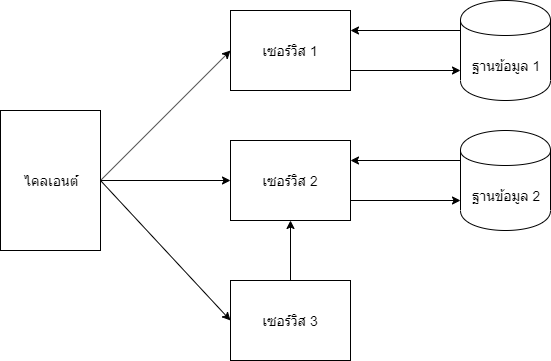
\includegraphics[width=0.7\textwidth]{microservices}  
		\caption{แผนผังแสดงตัวอย่างการออกแบบระบบโดยใช้สถาปัตยกรรมไมโครเซอร์วิส}
		\label{Fig:microservices}
	\end{figure}

	\item \textbf{REST (Representational state transfer)}

	REST เป็นสถาปัตยกรรมซอฟต์แวร์อย่างหนึ่งในการสร้างเว็บเซอร์วิส ทำให้แต่ละเซอร์วิสสามารถทำงานร่วมกันได้ผ่านเครือข่ายอินเตอร์เน็ต มักจะใช้ HTTP (Hypertext Transfer Protocol) เป็นโปรโตคอลในการสื่อสาร โดย HTTP นั้นเป็นโปรโตคอลแบบ Stateless ทำให้มีสมรรถภาพสูง, มีความน่าเชื่อถือ และมีความสามารถในการนำกลับไปใช้ใหม่ได้โดยไม่กระทบกับระบบส่วนอื่นแม้ว่าระบบกำลังทำงานอยู่ก็ตาม ~\cite{rest}
	
	\item \textbf{HTTP (Hypertext Transfer Protocol)}
	
	HTTP เป็นโปรโตคอลในการส่งข้อมูลบนเว็บ เป็นโปรโตคอลแบบไคลเอนต์-เซิร์ฟเวอร์ โดยไคลเอนต์จะส่งคำร้องขอข้อมูลไปยังเซิร์ฟเวอร์ จากนั้นเซิร์ฟเวอร์ก็จะส่งคำตอบกลับมาที่ไคลเอนต์ จากรูปที่ 2.2 จะเป็นตัวอย่างของการสื่อสารด้วยโปรโตคอล HTTP ~\cite{http}

	\begin{figure}[!h]
		\centering
		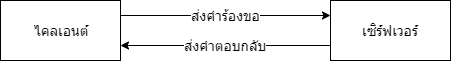
\includegraphics[width=0.7\textwidth]{http}  
		\caption{แผนผังแสดงตัวอย่างการสื่อสารด้วยโปรโตคอล HTTP}
		\label{Fig:http}
	\end{figure}

	\item \textbf{Repository Pattern}
	
	Repository Pattern เป็นรูปแบบหนึ่งในการออกแบบเซอร์วิส โดย Repository เป็นคลาสที่ห่อหุ้มลอจิกต่าง ๆ ที่เอาไว้เข้าถึงแหล่งข้อมูล ทำให้สามารถเข้าถึงข้อมูลเพียงแค่ใช้ฟังก์ชัน, ง่ายต่อการดูแลรักษา และแยกส่วนการทำงานระหว่างเทคโนโลยีที่เอาไว้เข้าถึงแหล่งข้อมูลออกจากโดเมนเลเยอร์ของโมเดล ~\cite{repositorypattern} จากตัวอย่างในรูปที่ 2.3 จะมีคลาสของออบเจ็กต์ชื่อว่า Product และออบเจ็กต์ถูกเก็บอยู่ในฐานข้อมูล เมื่อมีลอจิกทางธุรกิจใดก็ตามที่ต้องการค้นหา Product ตามชื่อที่ต้องการ เราสามารถใช้เมธอด findByName ของคลาส ProductRepository เพื่อทำการค้นคืนข้อมูลออบเจ็กต์ Product ที่เราต้องการได้ทันที
	
	\begin{figure}[!h]
		\centering
		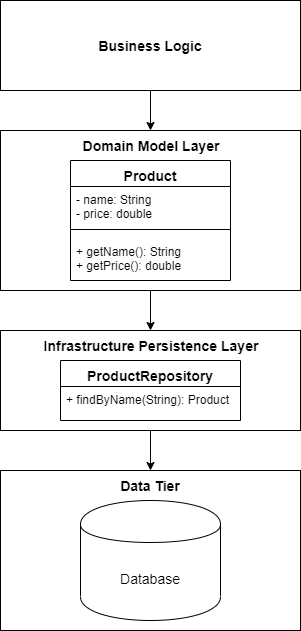
\includegraphics[width=0.495\textwidth]{repository}  
		\caption{แผนผังแสดงตัวอย่างของ Repository Pattern}
		\label{Fig:repository}
	\end{figure}
	
	\item \textbf{Object-Relational Mapper (ORM)}
	
	Object-Relational Mapper เป็นการแปลงออบเจ็กต์ที่เกิดขึ้นจากแนวคิดการเขียนโปรแกรมเชิงวัตถุ (Object-Oriented Programing) ให้สามารถใช้งานกับฐานข้อมูลประเภท Relational ได้ ~\cite{orm} ยกตัวอย่างเช่น คลาส Product มีคุณลักษณะต่าง ๆ ได้แก่ id, name และ price เมื่อนำ ORM มาใช้เพื่อแปลงออบเจ็กต์ของคลาสนี้ไปอยู่ในรูปของ Relation ก็จะได้ Relation ที่มีโครงสร้างดังรูปที่ 2.4
	
	\begin{figure}[!h]
		\centering
		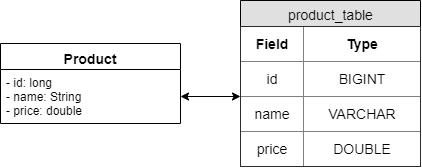
\includegraphics[width=0.65\textwidth]{orm}  
		\caption{ตัวอย่างการแปลงออบเจ็กต์ของคลาสไปเป็น Relation ด้วย Object-Relational Mapper}
		\label{Fig:orm}
	\end{figure}
	
	\item \textbf{คอนเทนเนอร์}
	
	คอนเทนเนอร์เป็นหน่วยของซอฟต์แวร์ที่ทำการบรรจุโค้ดและส่วนอื่น ๆ ที่เกี่ยวข้องเอาไว้ทั้งหมดเพื่อให้สามารถรันได้ทันทีในสภาพแวดล้อมใดก็ได้ มีความเป็นมาตรฐาน และประหยัดทรัพยากร เนื่องจากในการรันหลาย ๆ แอปพลิเคชันที่เป็นคอนเทนเนอร์พร้อมกันจะใช้แค่ระบบปฏิบัติการเดียว
	
	\begin{figure}[!h]
		\centering
		\subfigure[]{
			\label{Fig:infra:container}
			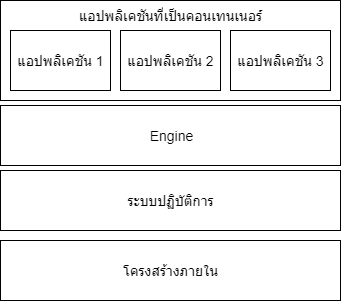
\includegraphics[width=0.45\textwidth]{container-infra}  
		}
		\subfigure[]{
			\label{Fig:infra:vm}
			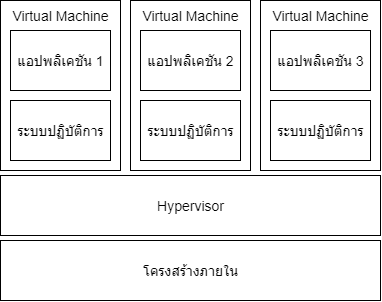
\includegraphics[width=0.5\textwidth]{vm-infra}  
		}
		\caption{แผนผังแสดงโครงสร้างเบื้องต้นภายในเซิร์ฟเวอร์เมื่อทำการใช้งานคอนเทนเนอร์ (ก) กับ Virtual Machine (ข)}
		\label{Fig:infra}
	\end{figure}

	จากรูป 2.5 แสดงให้เห็นว่า Virtual Machine ทั้งหมดจำเป็นต้องมีระบบปฏิบัติการเป็นของตนเอง ทำให้สิ้นเปลืองทรัพยากรของเซิร์ฟเวอร์โดยไม่จำเป็น แต่คอนเทนเนอร์สามารถรันร่วมกันได้โดยใช้ระบบปฏิบัติการร่วมกัน และมี Engine เป็นตัวจัดการการทำงานของแต่ละคอนเทนเนอร์ ทำให้ประหยัดทรัพยากรของเซิร์ฟเวอร์ และประหยัดค่าใช้จ่ายในเรื่องลิขสิทธิ์ของระบบปฏิบัติการที่ใช้รันเซิร์ฟเวอร์ ~\cite{container}
	
	\item \textbf{Orchestration}
	
	Orchestration เป็นตัวจัดการระบบคอมพิวเตอร์และซอฟต์แวร์ รวมไปการตั้งค่าต่าง ๆ และการประสานงานกับซอฟต์แวร์อื่น ๆ โดยอัตโนมัติ ~\cite{orchestration}
	
\end{enumerate}

\section{เครื่องมือและเทคโนโลยีที่ใช้ในการปฏิบัติงาน}
\begin{enumerate}
	\item \textbf{IntelliJ IDEA}
	
	IntelliJ IDEA เป็น Integrate Development Environment (IDE) สำหรับใช้ในการพัฒนาซอฟต์แวร์ที่ใช้ Java Virtual Machine (JVM) โดยเฉพาะ มีระบบแนะนำการเขียนโค้ดกับระบบเติมคำอัตโนมัติ ทำให้การเขียนโค้ดเป็นไปอย่างราบรื่นและรวดเร็ว โดยรูปที่ 2.6 จะเป็นตัวอย่างของระบบดังกล่าว ~\cite{intellij}
	
	\begin{figure}[!h]
		\centering
		\subfigure[]{
			\label{Fig:intellij:suggestion}
			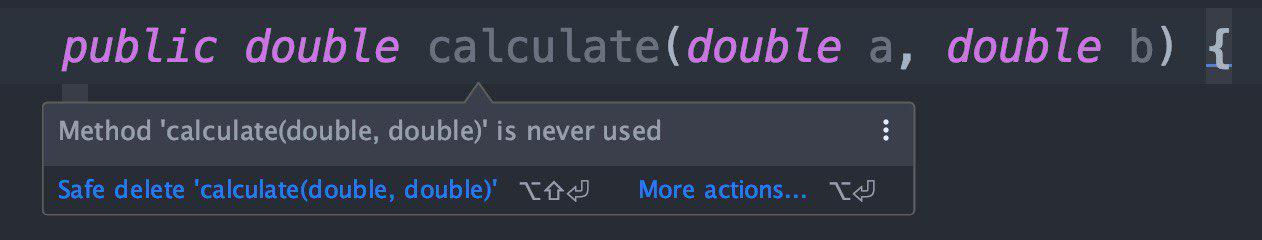
\includegraphics[width=0.8\textwidth]{suggestion}  
		}
		\subfigure[]{
			\label{Fig:intellij:auto-completion}
			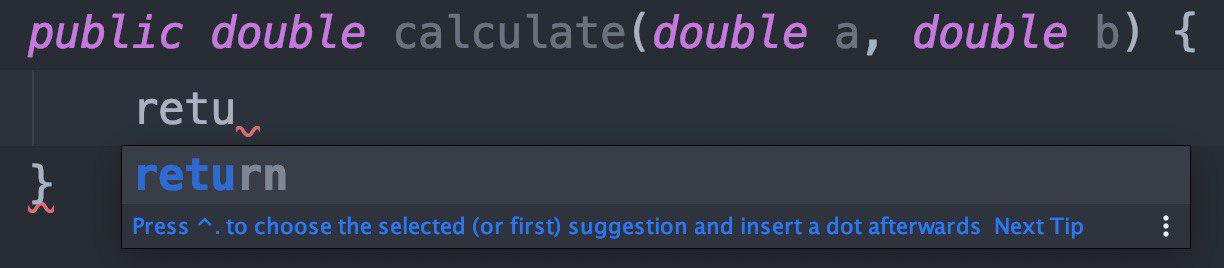
\includegraphics[width=0.8\textwidth]{auto-completion}  
		}
		\caption{ระบบแนะนำการเขียนโค้ด (ก) กับระบบเติมคำอัตโนมัติ (ข) ของ IntelliJ IDEA}
		\label{Fig:intellij}
	\end{figure}
	
	\item \textbf{Visual Studio Code}
	
	Visual Studio Code เป็น Text Editor ที่สามารถรองรับภาษาโปรแกรมมิ่งได้หลากหลายภาษา มีระบบไฮไลท์ Syntax ในการตรวจสอบ Syntax ของโค้ด ช่วยลดความผิดพลาดจากการเขียนโค้ดผิด Syntax ของภาษาโปรแกรมมิ่ง และสามารถติดตั้งส่วนขยายต่าง ๆ  เพิ่มเติมได้ตามความเหมาะสมในการทำงาน ~\cite{vscode}
	
	\item \textbf{Java}
	
	Java เป็นภาษาโปรแกรมมิ่งที่รองรับการเขียนโปรแกรมแบบ Object-Oriented เมื่อทำการคอมไพล์ไฟล์ .java แล้ว จะได้เป็น bytecode ออกมา โดยเราสามารถนำ bytecode ไปรันบนคอมพิวเตอร์เครื่องไหนก็ได้ที่ติดตั้ง Java Virtual Machine (JVM) ไว้ ~\cite{java}
	
	\item \textbf{Spring Boot}
	
	Spring Boot คือ เฟรมเวิร์คของภาษาโปรแกรมมิ่งที่ใช้ Java Virtual Machine (JVM) สำหรับช่วยในการพัฒนา REST API, Websocket, Web และอื่น ๆ โดยเฟรมเวิร์คนี้ถูกออกแบบมาเพื่อสร้างแอปพลิเคชันแล้วสามารถนำไปใช้ได้ทันที โดยที่ไม่จำเป็นต้องตั้งค่าอะไรเพิ่มเติม ~\cite{spring}
	
	\item \textbf{Hibernate ORM}
	
	Hiberate ORM คือ เฟรมเวิร์ค Object Relation Mapping ที่จะแปลงออบเจกต์ให้ใช้งานกับฐานข้อมูลประเภท Relational ได้โดยผ่านทาง JDBC (Java Database Connectivity) ซึ่งเป็น API สำหรับภาษา Java เพื่อให้สามารถเข้าถึงฐานข้อมูลได้ ~\cite{hibernate}

	\item \textbf{Maven}
	
	Maven คือ ซอฟแวร์จัดการโปรเจค ช่วยลดขั้นตอนในการ Build ซอฟต์แวร์, ทำให้การ Build ซอฟต์แวร์เป็นมีระเบียบมากขึ้นโดยใช้ Project Object Model (POM) ซึ่งเป็นจะไฟล์ .xml ดังรูปที่ 2.7 เราสามารถตั้งค่าต่าง ๆ ให้กับโปรเจคและจัดการ Dependencies ที่เกี่ยวข้องกับโปรเจคโดยใช้ไฟล์ pom.xml ~\cite{maven}
	
	\begin{figure}[!h]
		\centering
		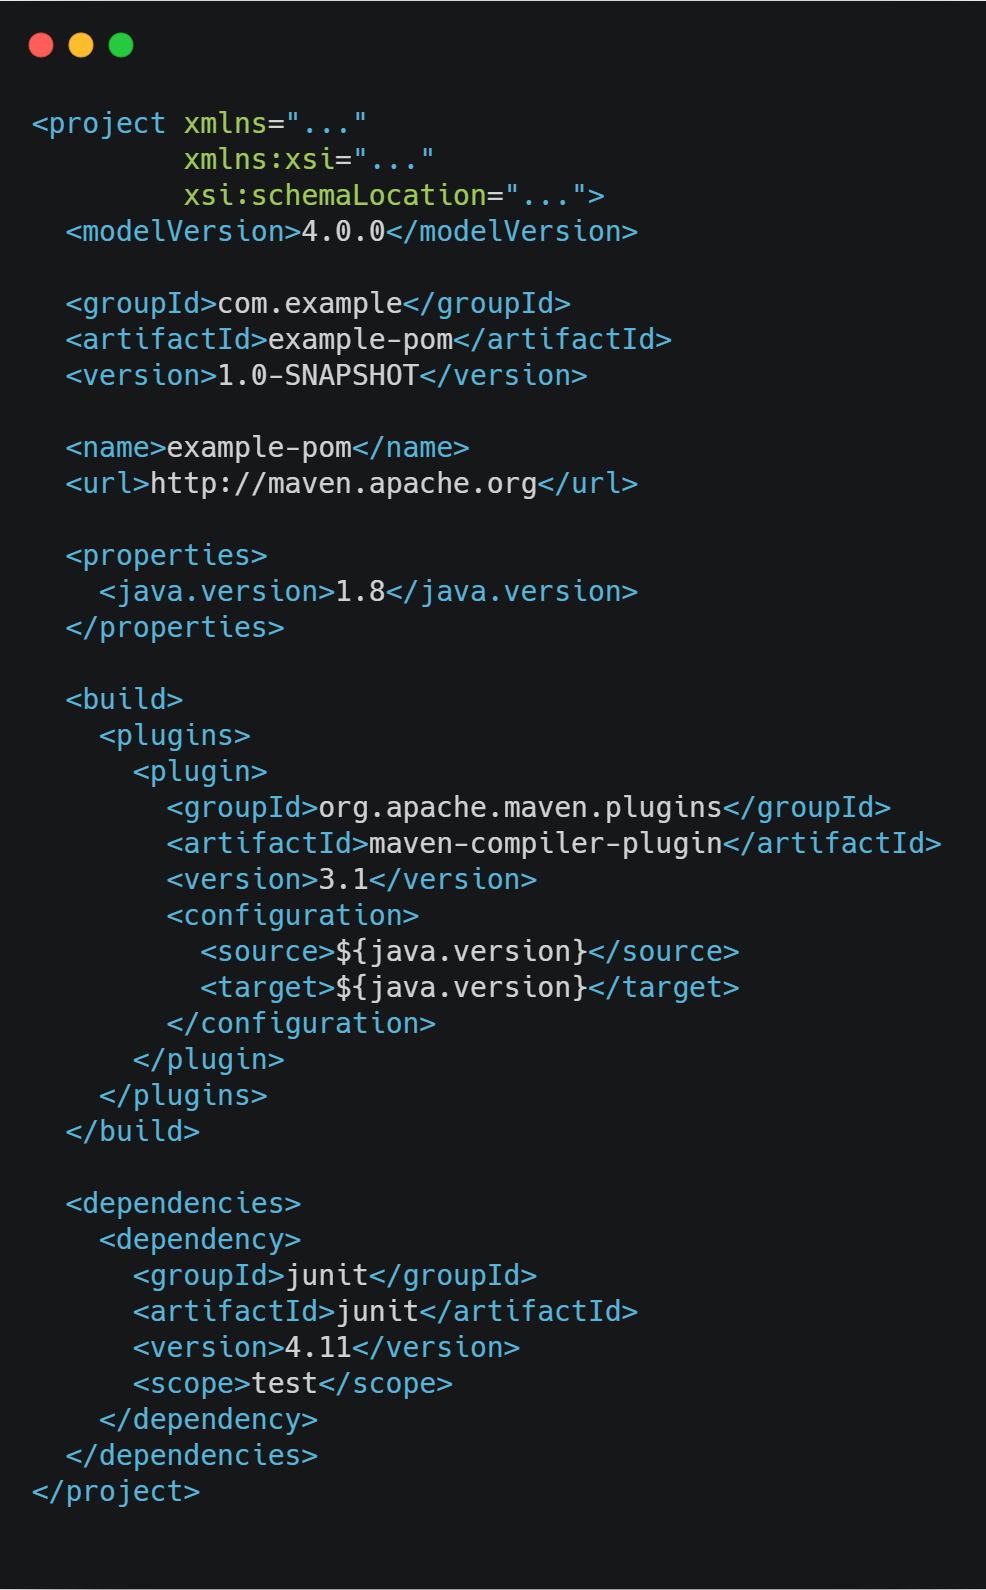
\includegraphics[width=0.695\textwidth]{pom}  
		\caption{ตัวอย่างไฟล์ pom.xml ของ Maven}
		\label{Fig:pom}
	\end{figure}
	
	\item \textbf{Python}
	
	Python เป็นภาษาโปรแกรมมิ่งที่เป็น Interpreter มีจุดเด่นที่สามารถอ่านและทำความเข้าใจโค้ดได้ง่ายและ Interpreter ของ Python นั้น สามารถติดตั้งได้ในหลายระบบปฏิบัติการ ~\cite{python}
		
	\item \textbf{MySQL}
	
	MySQL เป็นตัวจัดการฐานข้อมูลแบบ Relational ที่เป็น Open source ~\cite{mysql}
	
	\item \textbf{Google BigQuery}
	
	Google BigQuery เป็นบริการคลังข้อมูลบน Cloud ที่ให้บริการโดย Google และสามารถใช้ SQL เพื่อใช้งาน Google BigQuery ได้ ~\cite{bigquery}
	
	\item \textbf{Git}
	
	Git คือ Version Control ที่สามารถติดตามและควบคุมการเปลี่ยนแปลงของโค้ดได้ เพื่อให้ Software Engineer คนอื่น ๆ สามารถทำงานร่วมกันได้อย่างมีประสิทธิภาพ ~\cite{git}

	\item \textbf{Postman}
	
	Postman เป็นแอปพลิเคชันสำหรับสร้างคำร้องขอไปยังเซิร์ฟเวอร์ เช่น REST, SOAP, GraphQL เพื่อทดสอบการทำงาน API (Application Programming Interface) ของเซิร์ฟเวอร์ และสามารถตรวจสอบคำตอบกลับที่ส่งกลับมาได้ ~\cite{postman}
	
	\item \textbf{Docker}
	
	Docker คือ คอนเทนเนอร์ Engine สำหรับสร้างและจัดการคอนเทนเนอร์ของซอฟต์แวร์ ทำให้ซอฟต์แวร์สามารถนำไปใช้งานในสภาพแวดล้อมไหนก็ได้ ~\cite{docker} โดยเราสามารถตั้งค่าการสร้างคอนเทนเนอร์อิมเมจได้จาก Dockerfile หรือจะใช้อิมเมจสาธารณะจาก Docker Hub ก็ได้ จากรูปที่ 2.8 เป็นตัวอย่าง Dockerfile ที่จะสร้างอิมเมจที่สามารถรันแอปพลิเคชันที่สร้างจาก Node.js ได้ ซึ่งเป็นเฟรมเวิร์คหนึ่งของภาษา Javascript ในการสร้างเน็ตเวิร์คแอปพลิเคชัน ~\cite{nodejs}
	
	\begin{figure}[!h]
		\centering
		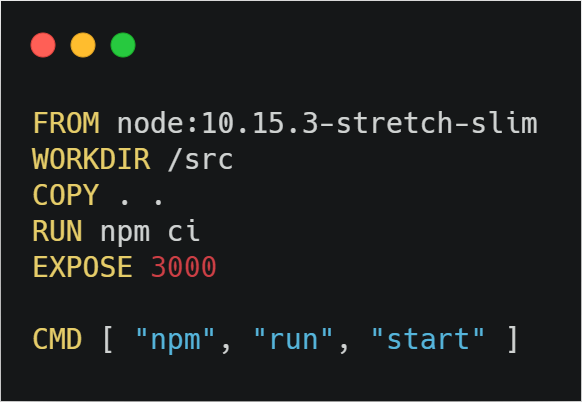
\includegraphics[width=0.5\textwidth]{dockerfile}  
		\caption{ตัวอย่างไฟล์ Dockerfile ที่ใช้ในการตั้งค่าเพื่อสร้างอิมเมจของคอนเทนเนอร์}
		\label{Fig:dockerfile}
	\end{figure}
	
	\item \textbf{Kubernetes}
	
	Kubernetes คือ Orchestration ของกลุ่มคอนเทนเนอร์และกลุ่มเซิร์ฟเวอร์ มีความสามารถในการจัดการคอนเทนเนอร์ให้สามารถทำงานได้อย่างต่อเนื่อง มีช่วงเวลาหยุดทำงานเป็นศูนย์ 	 ~\cite{kubernetes} โดย Kubernetes ยังมีฟังก์ชันอำนวยความสะดวกอื่น ๆ เช่น
	\begin{itemize}
		\item กระจายโหลดที่เข้ามายังคอนเทนเนอร์ เพื่อให้สามารถทำงานได้อย่างมีเสถียรภาพ
		\item ตั้งค่าให้ Kubernetes จัดสรรทรัพยากรต่าง ๆ กับคอนเทนเนอร์ได้ เช่น หน่วยความจำ และหน่วยประมวลผล เป็นต้น โดย Kubernetes จะจัดการเพื่อให้คอนเทนเนอร์ทำงานได้เต็มประสิทธิภาพตามทรัพยากรที่กำหนดไว้
		\item เริ่มต้นการทำงานของคอนเทนเนอร์ที่หยุดทำงานให้ใหม่ สับเปลี่ยนคอนเทนเนอร์ ลบคอนเทนเนอร์ที่ไม่มีการตอบสนอง และจะไม่อนุญาตให้ใช้งานคอนเทนเนอร์ ถ้าไม่อยู่ในสถานะพร้อมใช้งานจริง ๆ
		\item เก็บข้อมูลความลับต่าง ๆ ได้ โดยสามารถ Deploy และอัปเดตข้อมูลลับและการตั้งค่า โดยที่ไม่ต้อง Build คอนเทนเนอร์ใหม่
	\end{itemize}
	ในการตั้งค่าต่าง ๆ ให้กับ Kubernetes สามารถทำได้ผ่านไฟล์ .yaml หรือ .yml ซึ่งเป็นภาษามาตรฐานของชุดข้อมูลสำหรับทุกภาษาโปรแกรมมิ่ง ~\cite{yaml} โดยรูปที่ 2.9 จะเป็นตัวอย่างของไฟล์ .yaml ที่เอาไว้ตั้งค่า Kubernetes
	
	\begin{figure}[!h]
		\centering
		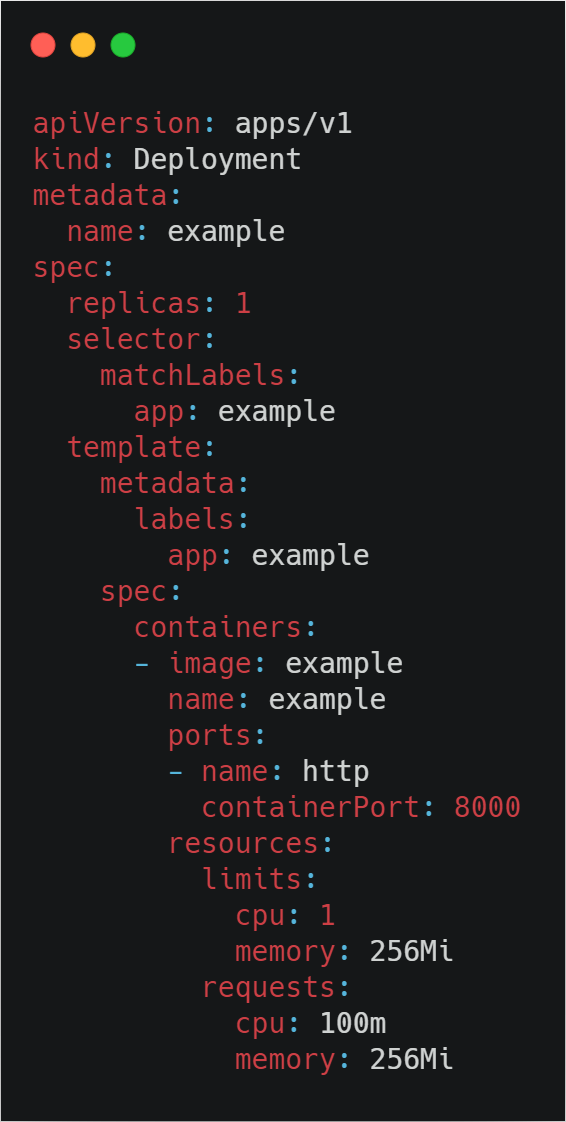
\includegraphics[width=0.375\textwidth]{k8sconfig}  
		\caption{ตัวอย่างไฟล์ .yml หรือ .yaml ในการตั้งค่าให้กับ Kubernetes}
		\label{Fig:cicdyaml}
	\end{figure}
	
	\item \textbf{Gitlab CI/CD}
	
	Gitlab CI/CD คือ เครื่องมือในการ Build ซอฟต์แวร์และ Deploy โดยอัตโนมัติ โดยเราสามารถตั้งค่าการทำงานของ Gitlab CI/CD ได้จากไฟล์ .gitlab-ci.yml ดังรูปที่ 2.10 ~\cite{gitlabcicd} 
	
	\begin{figure}[!h]
		\centering
		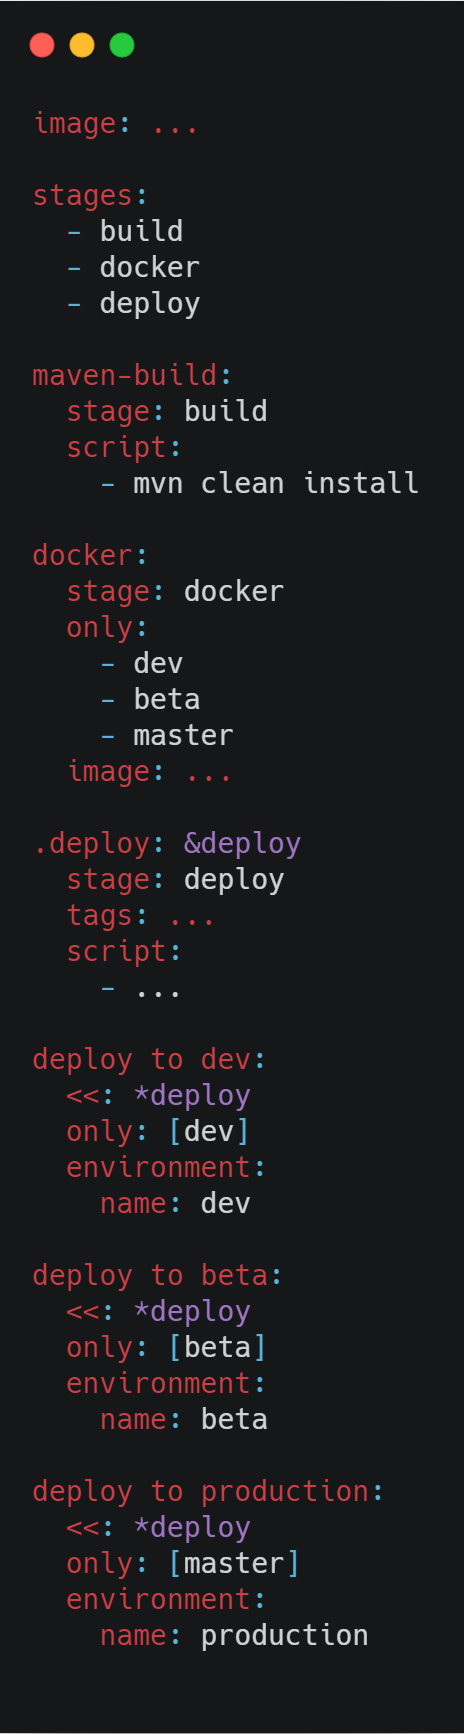
\includegraphics[width=0.375\textwidth]{cicdyaml}  
		\caption{ตัวอย่างไฟล์ .gitlab-ci.yml ในการตั้งค่าให้กับ Gitlab CI/CD}
		\label{Fig:cicdyaml}
	\end{figure}		
\end{enumerate}

\section{ลักษณะขั้นตอนการทำงาน}
ทีม Development ของบริษัท วงใน มีเดีย จำกัด (สำนักงานใหญ่) จะถูกแบ่งออกเป็นทีมย่อย ๆ ตามประเภทของงานที่รับผิดชอบ เรียกว่า Squad ซึ่งจะเป็นทีมแบบ Cross-Functional กล่าวคือ ภายในทีมจะประกอบไปด้วยหลาย ๆ ฝ่าย ได้แก่ Project Manager, UX/UI Designer, Software Engineer (Frontend), Software Engineer (Backend), Software Engineer (iOS), Software Engineer (Android) และ Quality Assurance Engineer โดยแต่ละ Squad อาจจะฝ่ายอื่น ๆ เพิ่มเติมแตกต่างกันไป ขึ้นอยู่กับลักษณะของงานที่รับผิดชอบ โดยแต่ละ Squad นั้นจะทำงานโดยใช้ Scrum Framework เป็นหลัก Scrum จะทำงานเป็นวงรอบ (Sprint) แต่ละรอบนั้นจะเท่ากับ 2 สัปดาห์ ภายใน Sprint จะกิจกรรมที่สำคัญต่าง ๆ ดังต่อไปนี้
\begin{enumerate}
	\item \textbf{Sprint Planning}
	
	เป็นการประชุมตอนต้น Sprint เพื่อรับมอบหมายงานจาก Project Manager และเป็นการประชุมเพื่อปรึกษาหาวิธีการทำงานและวิธีการแก้ไขปัญหาต่าง ๆ ที่เกี่ยวกับงานที่ได้รับมอบหมาย
	
	\item \textbf{Daily Meeting}
	
	เป็นการประชุมแบบสั้น ๆ ประจำวัน มีจุดประสงค์เพื่อให้สมาชิกทีมรับทราบความคืบหน้าของงานที่แต่ละคนกำลังทำอยู่และทราบปัญหาที่เกิดขึ้นระหว่างการทำงาน
	
	\item \textbf{Backlog Refinement Meeting}
	
	ปกติเมื่อ Squad ได้รับมอบหมายให้ทำงานใหม่ ๆ งานนั้นจะถูกจัดไว้ใน Features Backlog ก่อน ซึ่งงานที่อยู่ในนี้จะถูกนำเข้า Sprint ถัด ๆ ไป ขึ้นอยู่กับการตัดสินใจของ Project Manager การประชุมนี้จะจัดตอนกลาง Sprint เพื่อพิจารณางานที่อยู่ Features Backlog ว่าควรจะทำอย่างไร, เป็นงานสำคัญที่ต้องเอามาเท่าก่อนหรือไม่ และประเมินเวลาที่จะต้องใช้ในการทำงานชิ้นนี้ เป็นต้น
	
	\item \textbf{Retrospective Meeting}
	
	เป็นการประชุมตอนปลาย Sprint เพื่อสรุปการทำงานที่ได้ทำไปในรอบ และให้สมาชิกภายในทีมอธิบายปัญหาที่เกิดขึ้นในรอบ รวมไปถึงเรื่องราวดี ๆ ที่เกิดขึ้นในรอบด้วย เพื่อนำไปปรับปรุงการทำงานในรอบถัดไป
\end{enumerate}

การติดต่อสื่อสารภายในองค์กรจะใช้โปรแกรม Slack เป็นหลัก ดังรูปที่ 2.11 ส่วนสถานะของงานภายในทีมสามารถดูได้จาก Kanban Board ดังรูปที่ 2.12 ซึ่งเป็นบอร์ดที่ตั้งอยู่ในพื้นที่ทำงาน หรือดูจาก Asana ที่ระบบออนไลน์ก็ได้ สำหรับการทำงานของทีม Development ของ Wongnai งานหนึ่งชิ้นจะมีสถานะของงาน ดังต่อไปนี้

\begin{enumerate}
	\item \textbf{To do}
	
	งานที่ยังไม่ได้เริ่มทำ แต่อยู่ใน Sprint แล้วจะมีสถานะเป็น To do
	
	\item \textbf{In progress}
	
	งานที่กำลังทำอยู่จะมีสถานะเป็น In progress
	
	\item \textbf{Review}
	
	เมื่องานที่ทำอยู่เสร็จแล้ว ก่อนที่จะนำงานส่วนที่ทำเข้าไปใน Beta Environment ของเซิฟเวอร์ ซึ่งเป็น Environment ที่มีไว้ทดสอบก่อนที่จะใช้งานจริง โค้ดที่เขียนขึ้นมาจะต้องผ่านการตรวจสอบจาก Software Engineer คนอื่นอย่างน้อย 2 คนก่อน จึงจะสามารถส่งไปให้ Quality Assurance Engineer ทำการทดสอบต่อได้
	
	\item \textbf{Review passed}
	
	เมื่องานที่ทำอยู่ผ่านการตรวจสอบโดย Software Engineer คนอื่นครบ 2 คนแล้ว งานจะอยู่ในสถานะ Review passed 
	
	\item \textbf{Testing}
	งานที่อยู่ในสถานะ Review passed จะถูกส่งต่อให้ Quality Assurance Engineer ทดสอบ ซึ่งก่อนที่จะให้ Quality Assurance Engineer ทดสอบนั้น จะต้องเตรียมวิธีการทดสอบและเตรียมข้อมูลให้เรียบร้อยก่อน
	
	\item \textbf{Test passed}
	
	เมื่อ Quality Assurance Engineer ทดสอบเสร็จแล้ว งานจะอยู่ในสถานะ Test passed สามารถนำงานเข้า Beta Environment ได้เลย
	
	\item \textbf{Done}
	
	เมื่อนำงานเข้าไปใน Beta Environment เสร็จแล้ว งานจะมีสถานะเป็น Done แต่อย่างไรก็ตาม เจ้าของงานจะต้องติดตามงานของตัวเองจนกว่างานจะขึ้นอยู่บนระบบที่ใช้งานจริง (Production Environment)
\end{enumerate}

โดยส่วนมากแล้ว ถ้าเป็นงานที่เป็นการเขียนโค้ดจะมีกระบวนการทำงานตามที่กล่าวมาข้างต้น แต่อย่างไรก็ตามงานบางชนิดไม่จำเป็นต้องทำตามกระบวนการอย่างเคร่งครัดก็ได้ ขึ้นอยู่กับความเหมาะสมของงานว่าควรจะเป็นแบบไหน และในการทำงานของทีม Development ที่เป็นการเขียนโค้ดจะใช้ Test Driven Development (TDD) เป็นหลัก เป็นการเขียนชุดทดสอบของโค้ดขึ้นมาก่อน แล้วรันชุดทดสอบให้เกิดข้อผิดพลาด จากนั้นจึงเขียนโค้ดเพื่อแก้ไขข้อผิดพลาดนั้น ระหว่างการเขียนโค้ดจะต้องคอยคำนึงถึงคุณภาพของโค้ด หากมีโค้ดส่วนที่ไม่จำเป็นกจะต้องทำการ Refactor โค้ดส่วนนั้นด้วย โดยการ Refactor จะเป็นการลบโค้ดส่วนที่ไม่จำเป็นออก และนำโค้ดส่วนอื่น ๆ มาใช้ซ้ำให้มากที่สุด เพื่อให้โค้ดสั้นลง, มีคุณภาพ และ Software Engineer คนอื่น สามารถพัฒนาโค้ดส่วนนี้ต่อได้ง่าย

\begin{figure}[!h]
	\centering
	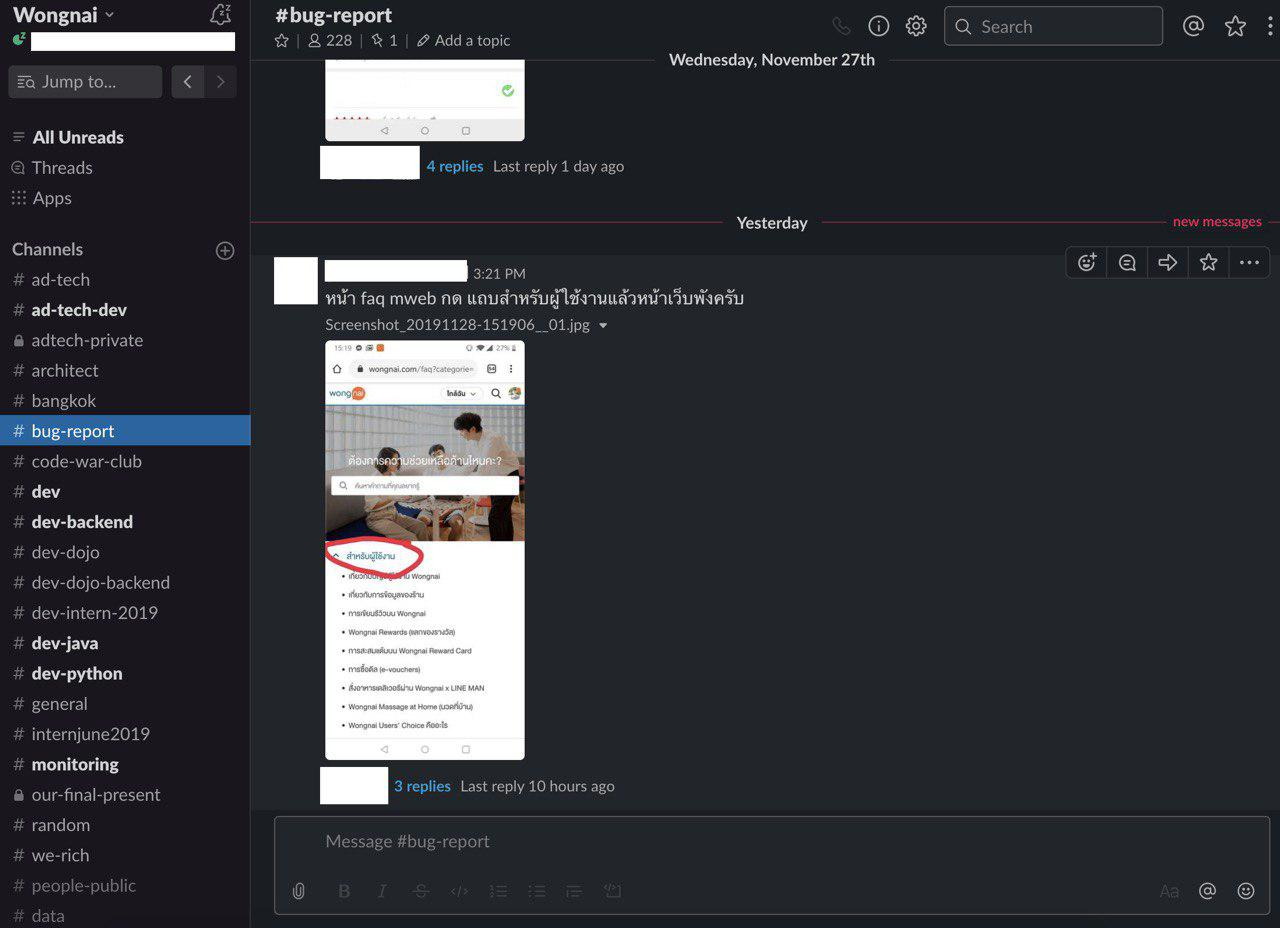
\includegraphics[width=1\textwidth]{slack}  
	\caption{ตัวอย่างของโปรแกรม Slack}
	\label{Fig:slack}
\end{figure}

\begin{figure}[!h]
	\centering
	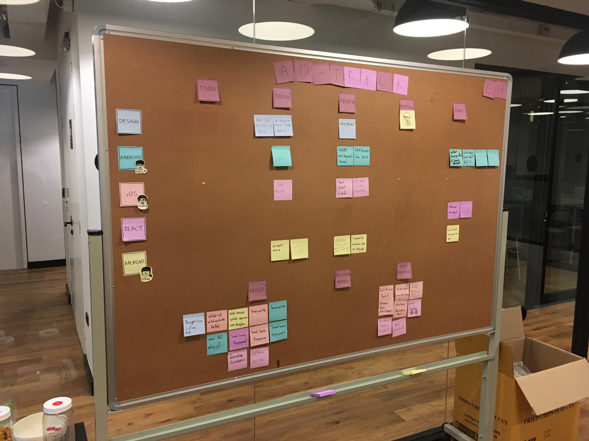
\includegraphics[width=1\textwidth]{kanban-board.png}  
	\caption{Kanban Board ที่ตั้งอยู่ในพื้นที่ทำงาน}
	\label{Fig:kanban-board}
\end{figure}
    \chapter{การออกแบบระบบ และรายละเอียดการพัฒนา}
\label{chapter:system-detail}
\section{ภาพรวมของระบบ}
การทำงานของระบบจัดการโฆษณาแบบจำกัดจำนวนการคลิกและการแสดงโฆษณา จะประกอบไปด้วยหลาย ๆ เซอร์วิสที่ทำงานร่วมกัน เพื่อให้สามารถทำงานได้ตามฟังก์ชันหลักที่จำเป็น ดังนี้

\begin{figure}[!h]
	\centering
	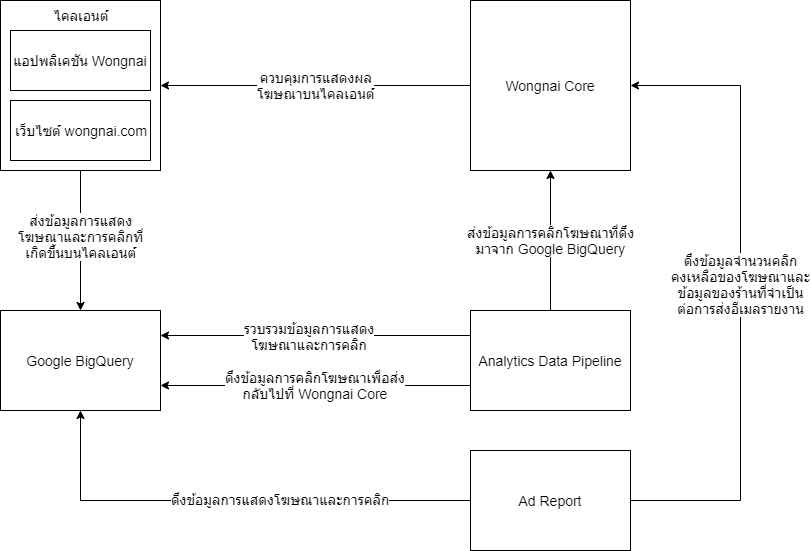
\includegraphics[width=1\textwidth]{ad-report-diagram.png}  
	\caption{แผนผังภาพรวมการทำงานของระบบจัดการโฆษณาแบบจำกัดจำนวนการคลิกและการแสดงโฆษณา}
	\label{Fig:adreport-diagram}
\end{figure}
	
โดย Wongnai Core เป็นเซอร์วิสขนาดใหญ่และเป็นเซอร์วิสหลักของ Wongnai ซึ่งเซอร์วิสนี้เคยเป็นเซอร์วิสที่มีสถาปัตยกรรมแบบ Monolith เมื่อนานมาแล้ว กล่าวคือระบบของ Wongnai ทุกอย่างเคยถูกพัฒนาใน Wongnai Core เพียงแค่ที่นี้ที่เดียว ไม่มีการแยกออกเป็นเซอร์วิสย่อย ๆ ภายหลังเมื่อระบบของ Wongnai มีขนาดใหญ่มากขึ้น แต่ละ Squad ไม่สามารถทำงานได้อย่างคล่องตัว จึงจำเป็นต้องแยกส่วนการทำงานออกมาเป็นอีกเซอร์วิสย่อยโดยใช้สถาปัตยกรรมไมโครเซอร์วิส อย่างไรก็ตามถ้าการแยกเซอร์วิสย่อยออกมา ไม่ทำให้ทีมทำงานได้คล่องตัวขึ้นเลย ก็ไม่จำเป็นจะต้องแยกเซอร์วิสก็ได้ สามารถพัฒนาฟังก์ชันใหม่ใน Wongnai Core ได้เลย ~\cite{wnservice}

ในการปฏิบัติงานนี้ ได้เล็งเห็นว่าหากเพิ่มฟังก์ชันที่สามารถส่งอีเมลรายงานผลการโฆษณากลับไปยังลูกค้าโดยอัตโนมัติได้ จะทำให้ Wongnai Core มีขนาดใหญ่เกินไป, การ Build เซอร์วิสนั้นนานมากขึ้น และเสียเวลาในการพัฒนาฟังก์ชันมากขึ้น จึงมีได้ตกลงกันว่าควรจะแยกออกเป็นอีกเซอร์วิสหนึ่ง ที่สามารถจัดการในเรื่องการส่งอีเมลรายงานผลการโฆษณากลับไปยังลูกค้าโดยอัตโนมัติโดยเฉพาะ แต่อย่างไรก็ตาม ระบบจัดการโฆษณาเดิมที่มีอยู่แล้ว อยู่ที่ Wongnai Core และมีความเห็นจาก Squad ว่า การนำฟังก์ชันส่วนนี้ออกมานั้นทำให้เสียเวลาในการพัฒนามากเกินไป จึงได้พัฒนาฟังก์ชันการจำกัดการแสดงโฆษณาของร้านด้วยจำนวนการคลิกโฆษณาไว้ที่ Wongnai Core เนื่องจากจำเป็นที่จะต้องมีทั้งการพัฒนาจากเซอร์วิสเดิม และการสร้างเซอร์วิสใหม่ จึงได้มีการแบ่งหน้าที่รับผิดชอบงานในส่วนต่าง ๆ ดังที่ปรากฏในตารางที่ 3.1

\begin{table}[!h]    
	\centering
	\begin{tabular}{|c|c|l|}
		\hline
		\textbf{เซอร์วิส} & \textbf{ผู้รับผิดชอบ} & \multicolumn{1}{c|}{\textbf{หมายเหตุ}} \\ \hline
		Wongnai Core & พนักงาน, นักศึกษา & \begin{tabular}[c]{@{}l@{}}นักศึกษารับผิดชอบในการพัฒนา API สำหรับให้\\ Ad Report ขอข้อมูลเพิ่มเติมในการสร้างรายงาน\end{tabular} \\ \hline
		Analytics Data Pipeline & พนักงาน, นักศึกษา & \begin{tabular}[c]{@{}l@{}}นักศึกษารับผิดชอบในการสร้างโปรเซสเซอร์แยก \\ข้อมูลเหตุการณ์ที่เกี่ยวกับโฆษณาบน Wongnai\end{tabular} \\ \hline
		Ad Report & พนักงาน, นักศึกษา & \begin{tabular}[c]{@{}l@{}}นักศึกษารับผิดชอบพัฒนาเซอร์วิสนี้เป็นส่วนใหญ่\\ โดยมี Software Engineer (Frontend) และ UX/UI\\ Designer เป็นผู้ช่วยเหลือในการสร้างรูปแบบของ \\อีเมลและรายงาน\end{tabular} \\ \hline
	\end{tabular}
	\caption{ตารางการแบ่งหน้าที่รับผิดชอบงานในส่วนต่าง ๆ ของระบบ}
	\label{Table:role}
\end{table}

\section{รายละเอียดการพัฒนาระบบ}
รายละเอียดของแต่ละเซอร์วิสที่เกี่ยวข้องกับระบบจัดการโฆษณาแบบจำกัดจำนวนการคลิกและการแสดงโฆษณา และรายละเอียดส่วนที่ได้พัฒนาเพิ่มขึ้นมา จะเป็นไปดังต่อไปนี้

\begin{enumerate}
	\item Wongnai Core
	
	Wongnai Core เป็นเซอร์วิสขนาดใหญ่และเป็นเซอร์วิสหลักของ Wongnai พัฒนาด้วยภาษา Java โดยหน้าที่ของ Wongnai Core ที่เกี่ยวข้องกับระบบจัดการโฆษณาแบบจำกัดจำนวนการคลิกและการแสดงโฆษณาโดยตรง ได้แก่
	
	\begin{itemize}
		\item จัดการโฆษณาที่แสดงบน Wongnai โดยสามารถจัดการได้จากหน้าแอดมินของ Wongnai Core ซึ่งเป็นหน้าแอดมินที่ใช้งานมานานแล้ว โดยจะเป็นหน้าแอดมินดังกล่าว จะถูกใช้โดยพนักงานที่เกี่ยวข้องกับการโฆษณาบน Wongnai สามารถเพิ่ม-ลบร้านที่จะลงโฆษณา, เลือกตำแหน่งที่จะแสดงโฆษณาบน Wongnai, สามารถแก้ไขข้อความโฆษณา และสามารถกำหนดช่วงเวลาที่จะแสดงโฆษณาได้
		\item ประมวลผลเมื่อได้รับข้อมูลจำนวนคลิกของโฆษณา เพื่อนำมาอัปเดตในฐานข้อมูลของ Wongnai Core จากนั้นจึงทำการพิจารณาว่าควรจะนำโฆษณาที่แสดงอยู่ออกหรือไม่ โดยดูจากจำนวนคลิกของโฆษณาว่าเกินกว่าที่จำกัดไว้ตามที่ตกลงกันหรือไม่ ถ้าเกินก็จะหยุดการแสดงโฆษณานั้น ๆ
		\item รอรับการร้องขอข้อมูลจากเซอร์วิส Ad Report เพื่อนำข้อมูลไปใช้ในการสร้างรายงานที่สมบูรณ์ส่งกลับไปยังเจ้าของโฆษณา ซึ่งประกอบไปด้วย ชื่อร้าน, อีเมลของร้าน, จำนวนคลิกโฆษณาของร้านที่ใช้ไปแล้ว และจำนวนคลิกโฆษณาของร้านซื้อไว้
	\end{itemize}

	สำหรับส่วนที่ได้รับผิดชอบโดยตรงคือ การสร้าง API ใน Wongnai Core เพื่อให้เซอร์วิส Ad Report สามารถขอข้อมูลเพิ่มเติมในการส่งอีเมลรายงานผลการโฆษณา ในที่นี้ได้ใช้โปรโตคอล HTTP เป็นตัวกลางในการสื่อสาร โดยรายละเอียดของ API ที่ได้พัฒนาเพิ่มขึ้นมา จะเป็นไปดังต่อไปนี้
	
	\begin{itemize}
		\item API สำหรับดึงข้อมูลของร้าน
		
		\begin{table}[!h]
			\centering
			\begin{tabular}{|c|c|c|c|}
				\hline
				\textbf{API Name} & \textbf{Method} & \multicolumn{2}{c|}{\textbf{URL}} \\ \hline
				businessInformation & GET & \multicolumn{2}{c|}{https://\{url\}/cb/\_/listing-ads/business/\{businessId\}} \\ \hline
				\multicolumn{4}{|c|}{\textbf{Request Path Parameter}} \\ \hline
				\textbf{Parameter Name} & \textbf{M/O} & \textbf{SV/MV} & \textbf{Data Type} \\ \hline
				businessId & M & SV & String \\ \hline
				\multicolumn{4}{|c|}{\textbf{Response Parameter}} \\ \hline
				\textbf{Parameter Name} & \textbf{M/O} & \textbf{SV/MV} & \textbf{Data Type} \\ \hline
				businessName & M & SV & String \\ \hline
				businessEmail & O & SV & String \\ \hline
				\multicolumn{4}{|r|}{*M: Mandatory; O: Optional; *SV: Single value; MV: Multi Value;} \\ \hline
			\end{tabular}
			\caption{ตารางรายละเอียดของ API สำหรับดึงข้อมูลของร้าน}
			\label{Table:api-detail-1}
		\end{table}
		
		\item API สำหรับดึงข้อมูลจำนวนคลิกโฆษณาของร้าน
		
		\begin{table}[!h]
			\centering
			\begin{tabular}{|c|c|c|c|}
				\hline
				\textbf{API Name} & \textbf{Method} & \multicolumn{2}{c|}{\textbf{URL}} \\ \hline
				clickPackInformation & GET & \multicolumn{2}{c|}{https://\{url\}/cb/\_/listing-ads/current-used-click-pack/\{businessId\}} \\ \hline
				\multicolumn{4}{|c|}{\textbf{Request Path Parameter}} \\ \hline
				\textbf{Parameter Name} & \textbf{M/O} & \textbf{SV/MV} & \textbf{Data Type} \\ \hline
				businessId & M & SV & String \\ \hline
				\multicolumn{4}{|c|}{\textbf{Response Parameter}} \\ \hline
				\textbf{Parameter Name} & \textbf{M/O} & \textbf{SV/MV} & \textbf{Data Type} \\ \hline
				clickUsed & O & SV & String \\ \hline
				clickPuchased & O & SV & String \\ \hline
				\multicolumn{4}{|r|}{*M: Mandatory; O: Optional; *SV: Single value; MV: Multi Value;} \\ \hline
			\end{tabular}
			\caption{ตารางรายละเอียดของ API สำหรับดึงข้อมูลจำนวนคลิกโฆษณาของร้าน}
			\label{Table:api-detail-2}
		\end{table}
	\end{itemize}
		

	\item Analytics Data Pipeline
	
	Analytics Data Pipeline เป็นเซอร์วิสขนาดเล็กที่พัฒนาด้วยภาษา Python ปกติไคลเอนต์จะส่งข้อมูลเหตุการณ์ต่าง ๆ ที่เกิดขึ้นใน Wongnai มาเก็บใน Google BigQuery ซึ่งข้อมูลเหตุการณ์ต่าง ๆ นั้นมีหลายประเภทและมีปริมาณที่เยอะมากใน 1 วัน สาเหตุที่ใช้ Google BigQuery นั้นสืบเนื่องมาจากต้องการที่จะลดปัญหาจากปริมาณข้อมูลที่เยอะ ทำให้การดูแลรักษาฐานข้อมูล ทั้งในเรื่องของประสิทธิภาพและอื่น ๆ ทำได้ยากและมีค่าใช้จ่ายที่สูง โดย Google BigQuery เป็นเทคโนโลยีคลังข้อมูลที่ให้บริการอยู่บน Cloud ทำให้สามารถตัดปัญหาเรื่องการดูแลรักษาได้ทันที อย่างไรก็ตามข้อมูลเหตุการณ์ต่าง ๆ ที่ถูกส่งเข้ามาใน Google BigQuery จะถูกเก็บไว้ในตารางเดียวกันทั้งหมด ทำให้ตารางนั้นเป็นตารางที่มีข้อมูลมหาศาล และการดึงข้อมูลจาก Google BigQuery หนึ่งครั้ง จะต้องเสียค่าใช้จ่ายตามขนาดของข้อมูลในตาราง การดึงข้อมูลออกมาจากตารางใหญ่ โดยที่ใช้ข้อมูลเพียงแค่บางส่วนจะทำให้สูญเสียเครดิตไปโดยไม่จำเป็น Analytics Data Pipeline จึงถูกพัฒนาขึ้นเพื่อแก้ไขปัญหาในจุดนี้ ภายในเซอร์วิสนี้จะประกอบไปด้วยโปรเซสเซอร์ต่าง ๆ ซึ่งเป็นคลาสที่เอาไว้แยกข้อมูลแต่ละประเภทออกจากตารางใหญ่ สำหรับส่วนที่ได้รับผิดชอบโดยตรงคือ การเพิ่มโปรเซสเซอร์ที่สามารถแยกข้อมูลเหตุการณ์ที่เกี่ยวกับโฆษณาบน Wongnai โดยเราต้องทำการเพิ่มตารางใหม่ที่ต้องการใน Google BigQuery ก่อน จากนั้นจึงสร้างโปรเซสเซอร์ที่เอาไว้แยกข้อมูลขึ้นมา โดยจะต้องสร้าง Query String ที่เป็น SQL จากนั้นโปรเซสเซอร์ส่ง Query String ไปยัง Google BigQuery อีกที ซึ่ง Query String ที่จะใช้ จะเป็นการเลือกข้อมูลส่วนที่ต้องการออกมาก่อน เช่น "SELECT ... FROM ... WHERE ... GROUP BY ..." จากนั้นจึงนำข้อมูลส่วนที่แยกออกมาใส่ไปในตารางใหม่โดยใช้คำสั่ง "INSERT INTO ..."
	
	\begin{figure}[!h]
		\centering
		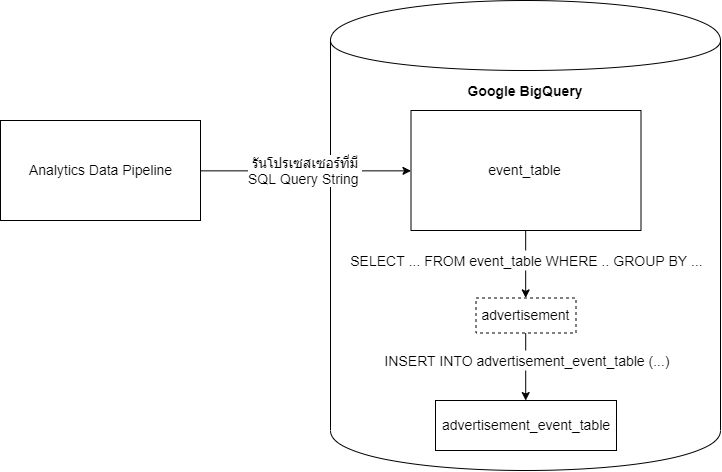
\includegraphics[width=0.95\textwidth]{analytics-data-pipeline}  
		\caption{แผนผังภาพรวมการทำงานของเซอร์วิส Analytics Data Pipeline}
		\label{Fig:analytics-data-pipeline}
	\end{figure}
	
	โปรเซสเซอร์ที่เพิ่มขึ้นมาจะทำให้ได้ตารางข้อมูลที่มีขนาดเล็กลง และมีเฉพาะส่วนที่เราต้องการนำไปใช้จริง ๆ ในที่นี้ได้เพิ่มโปรเซสเซอร์แยกเฉพาะข้อมูลเหตุการณ์ที่เกี่ยวกับโฆษณาบน Wongnai ออกมาเก็บไว้ในอีกตารางหนึ่งใน Google BigQuery เพื่อให้สะดวกต่อการนำไปใช้ต่อและลดค่าใช้จ่ายเนื่องจากไม่จำเป็นต้องไปดึงข้อมูลจากตารางใหญ่ โดยโปรเซสเซอร์นี้จะถูกรันทุก ๆ หนึ่งวันเพื่อเป็นการอัปเดตข้อมูลในตารางเล็กให้ทันปัจจุบัน
	
	\begin{table}[!h]
		\centering
		\begin{tabular}{|c|c|c|}
			\hline
			\textbf{Field name} & \textbf{Data Type} & \textbf{Description} \\ \hline
			Timestamp & TIMESTAMP & วันเวลาที่เกิดเหตุการณ์ \\ \hline
			EventLabel & STRING & ID ของร้าน \\ \hline
			EventAction & STRING & \begin{tabular}[c]{@{}c@{}}ประเภทของเหตุการณ์ที่เกิดขึ้น\\ ได้แก่ Click กับ Impression\end{tabular} \\ \hline
			App & STRING & \begin{tabular}[c]{@{}c@{}}Platform ที่เกิดเหตุการณ์ ได้แก่\\ Web, iOS และ Android\end{tabular} \\ \hline
			SearchResultView & STRING & \multirow{4}{*}{ตำแหน่งที่เกิดเหตุการณ์} \\ \cline{1-2}
			BusinessLandingDomain & STRING &  \\ \cline{1-2}
			Section & STRING &  \\ \cline{1-2}
			ScreenName & STRING &  \\ \hline
			Count & INTEGER & จำนวนครั้งที่เกิดเหตุการณ์ \\ \hline
		\end{tabular}
		\caption{Schema ของตารางที่แยกออกมาเพื่อเก็บข้อมูลเหตุการณ์ที่เกี่ยวกับโฆษณาบน Wongnai}
		\label{Table:schema-ad}
	\end{table}
		
	วิธีการตั้งค่าให้โปรเซสเซอร์ทำงานทุกวันโดยอัตโนมัติ จะใช้วิธีการทำ Task โดยอัตโนมัติด้วย CronJob ที่ Kubernetes ได้ โดยการเขียนไฟล์ .yaml ที่เอาไว้ตั้งค่าให้กับ Kubernetes 
	
	\begin{figure}[!h]
	 	\centering
	 	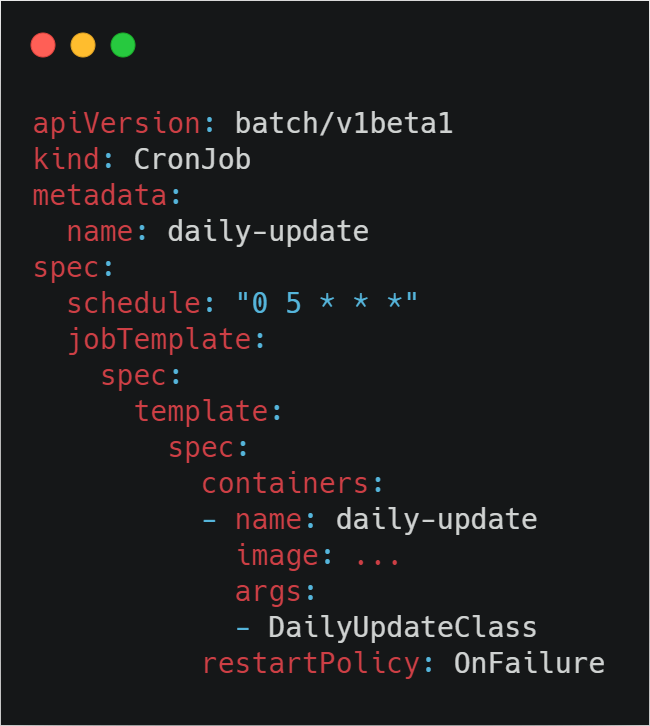
\includegraphics[width=0.475\textwidth]{cronjob1}  
	 	\caption{ตัวอย่างการตั้งค่า Kubernetes ให้รัน Task โดยอัตโนมัติด้วย CronJob}
	 	\label{Fig:cronjob1}
	\end{figure}
 
 	เราสามารถให้ตั้งค่า Kubernetes ให้รัน Task โดยอัตโนมัติได้ด้วย CronJob โดยตั้งเวลาที่ต้องการได้ที่ฟิลด์ schedule จากตัวอย่างรูปที่ 3.3 ได้ตั้งไว้ให้รันทุก ๆ วันตอน 13.00 น. เวลาประเทศไทย จุดสังเกตที่สำคัญคือ การตั้งเวลาต้องสังเกตด้วยว่าเครื่องที่เป็นเซิร์ฟเวอร์ที่จะรัน Task ใช้เขตเวลาอะไร ในที่นี้เขตเวลาของเครื่องจะเป็น UTC+0 จึงต้องคำนวณเวลาก่อนที่จะตั้งค่าลงไปในฟิลด์ schedule นอกจากนี้ หน้าที่อีกอย่างหนึ่งที่สำคัญของเซอร์วิสนี้ คือการนำข้อมูลเหตุการณ์ที่เกี่ยวกับโฆษณาบน Wongnai ที่แยกออกไปเก็บในตารางขนาดเล็กแล้ว ส่งไปอัปเดตที่ฐานข้อมูลของ Wongnai Core ทุก ๆ วัน เพื่อให้ Wongnai Core นำข้อมูลส่วนนี้ไปประมวลผลต่อตามที่กล่าวไว้ด้านบน
	
	\item Ad Report
	
	Ad Report เป็นเซอร์วิสใหม่ที่ถูกพัฒนาด้วยภาษา Java ร่วมกับ Spring Boot ทำหน้าที่สร้างอีเมลรายงานผลการโฆษณาที่ประกอบไปด้วยข้อมูลต่าง ๆ โดยภายในเซอร์วิสนี้ จะประกอบไปด้วยฟังก์ชันการทำงานหลัก 4 อย่าง ได้แก่
	\begin{itemize}
		\item Statistics Updater
		
		ฟังก์ชัน Statistics Updater ทำหน้าที่ดึงข้อมูลเหตุการณ์ที่เกี่ยวกับโฆษณาบน Wongnai ที่เก็บไว้อยู่ใน Google BigQuery มาอัปเดตลงในฐานข้อมูลของ Ad Report โดยฟังก์ชันนี้จะทำการส่ง Query String ที่เป็น SQL ไปยังตารางขนาดเล็กที่เก็บข้อมูลเหตุการณ์ที่เกี่ยวกับโฆษณาใน Google BigQuery เพื่อนำข้อมูลในช่วงเวลาที่ต้องการออกม าจากนั้นนำข้อมูลที่ได้มาบันทึกลงในฐานข้อมูล โดย Schema ของตารางที่จะบันทึกข้อมูลเหตุการณ์ที่เกี่ยวกับโฆษณาในเซอร์วิส Ad Report จะเป็นไปดังต่อไปนี้
		
		\begin{table}[!h]
			\centering
			\begin{tabular}{|c|c|c|}
				\hline
				\textbf{Field name} & \textbf{Data Type} & \textbf{Description} \\ \hline
				id & BIGINT & ID ของเหตุการณ์ \\ \hline
				timestamp & DATETIME & วันเวลาที่เกิดเหตุการณ์ \\ \hline
				business\_id & BIGINT & ID ของร้านที่เกิดเหตุการณ์ \\ \hline
				number\_of\_impressions & BIGINT & จำนวนครั้งที่แสดงโฆษณาของร้าน \\ \hline
				number\_of\_clicks & BIGINT & จำนวนครั้งที่เกิดการคลิกไปที่โฆษณาของร้าน \\ \hline
			\end{tabular}
			\caption{Schema ของตารางที่เก็บข้อมูลเหตุการณ์ที่เกี่ยวกับโฆษณาบน Wongnai ในเซอร์วิส Ad Report}
			\label{Table:schema-ad-report-1}
		\end{table}
		
		กรณีที่ข้อมูลที่เข้ามาใหม่จากการอัปเดตเป็นข้อมูลของร้านที่ไม่เคยปรากฏอยู่ในฐานข้อมูลของ Ad Report (เป็นร้านที่ลงโฆษณากับ Wongnai เป็นครั้งแรก) ฟังก์ชันนี้ก็จะทำการเรียกใช้งานฟังก์ชัน Retrieve Data เพื่อร้องขอข้อมูลชื่อร้านและอีเมลของร้านที่เข้ามาใหม่จาก Wongnai Core จากนั้นจึงบันทึกข้อมูลของร้านที่ได้มาทั้งหมดลงในอีกตาราง ซึ่งตารางนี้จะทำหน้าที่ในการเก็บข้อมูลของร้านเพื่อนำไปประกอบในการสร้างรายงานและการส่งอีเมล 
		
		\begin{table}[!h]
			\centering
			\begin{tabular}{|c|c|c|}
				\hline
				\textbf{Field name} & \textbf{Data Type} & \textbf{Description} \\ \hline
				business\_id & BIGINT & ID ของร้าน \\ \hline
				business\_name & VARCHAR(255) & ชื่อร้าน \\ \hline
				business\_email & VARCHAR(255) & อีเมลของร้าน \\ \hline
			\end{tabular}
			\caption{Schema ของตารางที่เก็บข้อมูลร้านในเซอร์วิส Ad Report}
			\label{Table:schema-ad-report-2}
		\end{table}
		
		\item Report
		
		ฟังก์ชัน Report ทำหน้าที่สร้างรายงานที่จะส่งไปพร้อมกับอีเมลให้กับลูกค้า โดยฟังก์ชันนี้จะทำการสร้างรายงานเป็นไฟล์นามสกุล .pdf จากเทมเพลตของรายงานที่เตรียมไว้ โดยเทมเพลตของรายงานจะเป็นไฟล์ที่ถูกแก้ไขมาแล้วบางส่วนให้ตรงกับที่ UX/UI Designer ออกแบบไว้ ซึ่งการจัดการไฟล์ .pdf จะใช้ไลบรารี iText ~\cite{itext} มาช่วยในการทำงาน ส่วนการสร้างแผนภูมิจะใช้ไลบรารี XChart  ~\cite{xchart} สำหรับการทำงานของฟังก์ชัน Report นั้น จะเป็นไปตามรูปที่ 3.4
		
		\begin{figure}[!h]
			\centering
			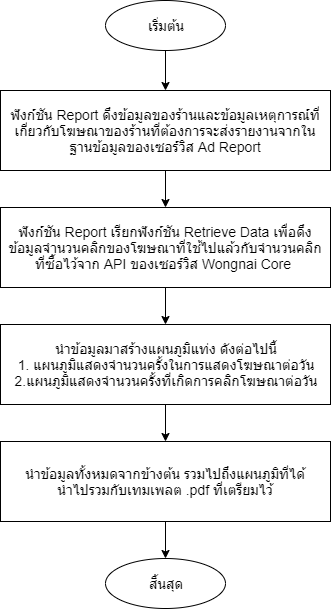
\includegraphics[width=0.5\textwidth]{report-diagram}  
			\caption{แผนผังการทำงานของฟังก์ชัน Report}
			\label{Fig:report-diagram}
		\end{figure}
		
		\item Report Email
		
		ฟังกชัน Report Email ทำหน้าที่สร้างอีเมลพร้อมกับแนบไฟล์รายงานที่ได้จากฟังก์ชัน Report ส่งไปยังอีเมลของลูกค้า ในที่นี้ได้ใช้คลาส EmailService ซึ่งเป็นคลาสที่มีอยู่แล้วในเฟรมเวิร์คของทาง Wongnai เพื่อทำการส่งอีเมล และใช้ Rocker Templates by Fizzed เป็นเทมเพลตสำหรับการเขียนอีเมลด้วย HTML ที่สามารถใช้คู่กับภาษา Java ได้ และมีประสิทธิภาพที่สูงในแง่ของความเร็วในการเรนเดอร์เทมเพลต ~\cite{rocker}
			
		\begin{figure}[!h]
			\centering
			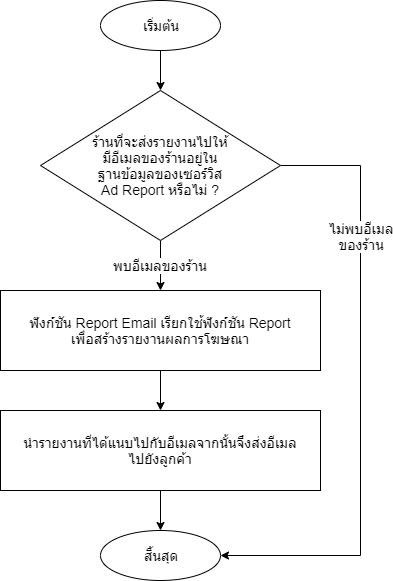
\includegraphics[width=0.65\textwidth]{email-diagram}  
			\caption{แผนผังการทำงานของฟังก์ชัน Report Email}
			\label{Fig:email-diagram}
		\end{figure}
			
		\item Retrieve Data
		
		ฟังกชัน Retrieve Data ทำหน้าหน้าที่ร้องขอข้อมูลที่จำเป็นจาก Wongnai Core เพื่อนำไปใช้ในการสร้างรายงานและการส่งอีเมลที่สมบูรณ์ โดยภายในฟังก์ชันนี้จะใช้คลาส RestTemplate ที่เป็นคลาสที่มีให้ในเฟรมเวิร์ค Spring Boot สำหรับการสร้างคำร้องขอแบบ REST ไปยัง API ของ Wongnai Core ทั้ง 2 API ได้แก่ API สำหรับดึงข้อมูลของร้าน กับ API สำหรับดึงข้อมูลจำนวนคลิกโฆษณาของร้าน ซึ่งได้อธิบายไว้แล้วก่อนหน้า
	\end{itemize}

	ภายในเซอร์วิส Ad Report จะมีคลาสที่เป็น ApplicationRunner อยู่อีกสองคลาส นอกเหนือจาก ApplicationRunner หลักที่เอาไว้รันเซอร์วิส Ad Report ถูกสร้างขึ้นมาเพื่อใช้ในการรัน Task โดยอัตโนมัติด้วย CronJob ที่ Kubernetes โดยทั้งสองคลาสจะมีรายละเอียดดังต่อไปนี้

	\begin{itemize}
		\item Weekly Report Email
		
		Weekly Report Email  เป็น ApplicationRunner Class ที่จะเรียกใช้งานฟังก์ชัน Report Email เพื่อสร้างรายงานผลการโฆษณาและส่งอีเมลกลับไปยังลูกค้าทุก ๆ สัปดาห์ ซึ่งจะส่งให้เฉพาะร้านที่ยังจำนวนคลิกโฆษณาคงเหลืออยู่ (กรณีที่ไม่มีจำนวนคลิกโฆษณาคงเหลือจะไม่ส่งแบบอัตโนมัติให้ เพราะถือว่าเป็นร้านที่โฆษณาหมดอายุไปแล้ว) โดยดูจากข้อมูลที่ร้องขอมาจากฟังก์ชัน Retrieve Data
	
		\begin{figure}[!h]
			\centering
			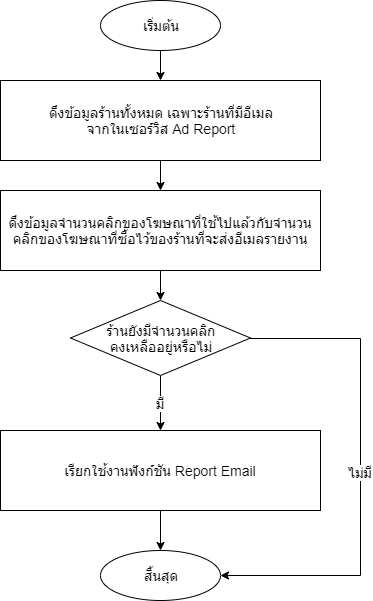
\includegraphics[width=0.55\textwidth]{weekly-report-email}  
			\caption{แผนผังการทำงานของ ApplicationRunner Class Weekly Report Email}
			\label{Fig:weekly-report-diagram}
		\end{figure}
	
		\item Daily Statistics Updater
	
		Daily Statistics Updater เป็น ApplicationRunner Class ที่จะเรียกใช้งานฟังก์ชัน Statistics Updater ทุก ๆ วัน เพื่ออัปเดตฐานข้อมูลเหตุการณ์ของโฆษณาบน Wongnai ของ Ad Report
	\end{itemize}

	นอกจากนี้เซอร์วิส Ad Report จะมีหน้าแอดมินสำหรับให้พนักงานที่เกี่ยวข้องมาใช้งานได้ โดยวิธีการพัฒนาหน้าแอดมินนั้นจะใช้เฟรมเวิร์ค admin-ui ที่ Wongnai มีให้อยู่แล้ว ซึ่ง admin-ui เป็นเฟรมเวิร์คที่ใช้ React ซึ่งเป็นไลบรารีสำหรับการสร้าง User Interface ให้กับเว็บไซต์ด้วยภาษา Javascript ~\cite{react} ถูกพัฒนามาสำหรับสร้างหน้าแอดมินให้กับเซอร์วิสใหม่ที่แยกออกมาจาก Wongnai Core โดยเราสามารถนำเฟรมเวิร์คนี้มาใช้ได้ทันที โดยที่ไม่จำเป็นต้องเขียนโค้ดอะไรเพิ่มเติมมากนัก แต่ในเซอร์วิส Ad Report นั้นต้องมี Action ในหน้าแอดมินที่สามารถส่งอีเมลรายงานด้วยตนเอง กรณีที่ระบบอัตโนมัติเกิดข้อผิดพลาดใด ๆ ก็ตาม ในการสร้าง Action ใน admin-ui จำเป็นต้องสร้าง API เพิ่มขึ้นมาในเซอร์วิส Ad Report โดย API ที่เพิ่มขึ้นมาจะทำการส่งอีเมลรายงานผลการโฆษณาให้กับลูกค้า ทันทีที่ได้รับการร้องขอ
	
	\begin{table}[!h]
		\centering
		\begin{tabular}{|c|c|c|c|}
			\hline
			\textbf{API Name} & \textbf{Method} & \multicolumn{2}{c|}{\textbf{URL}} \\ \hline
			sendWeeklyReportEmail & POST & \multicolumn{2}{l|}{\begin{tabular}[c]{@{}l@{}}https://\{url\}/admin/\\ business-information/\\ send-weekly-report-email/\\ \{buinessId\}\end{tabular}} \\ \hline
			\multicolumn{4}{|c|}{\textbf{Request Path Parameter}} \\ \hline
			\textbf{Parameter Name} & \textbf{M/O} & \textbf{SV/MV} & \textbf{Data Type} \\ \hline
			businessId & M & SV & String \\ \hline
		\end{tabular}
	\caption{ตารางรายละเอียดของ API สำหรับการสร้าง Action ส่งอีเมลรายงานผลการโฆษณาในหน้าแอดมิน}
	\label{Table:api-detail-3}
	\end{table}

	เฟรมเวิร์ค admin-ui จะคอยจัดการสิทธิ์การเข้าถึงหน้าแอดมินให้ โดยที่เราไม่จำเป็นต้องแนบพารามิเตอร์ใดเพิ่มเติม ๆ เข้าไปในคำร้องขอเพื่อยืนยันสิทธิ์การเข้าถึงหน้าแอดมิน เมื่อเราทำการส่งคำร้องขอไปที่ API นี้แล้ว ถ้าส่งอีเมลสำเร็จ จะได้คำตอบกลับ HTTP ที่มีสถานะเป็น 200 OK กลับมา แต่ถ้าไม่สำเร็จจะได้คำตอบกลับที่มีสถานะเป็น 4XX หรือ 5XX กลับมา ขึ้นอยู่กับว่าภายในเกิดข้อผิดพลาดอะไร
\end{enumerate}

เซอร์วิสทั้งหมดที่กล่าวมาทั้งหมดจะถูกทำให้เป็นคอนเทนเนอร์โดยใช้ Docker เพื่อให้สะดวกต่อการ Deploy ด้วย Kubernetes โดยแต่ละเซอร์วิสก็จะมี Dockerfile ไว้สำหรับการสร้างคอนเทนเนอร์อิมเมจของเซอร์วิสนั้น ๆ สำหรับ Ad Report ซึ่งเป็นเซอร์วิสใหม่นั้น ได้ทำการเพิ่มไฟล์ .gitlab-ci.yml สำหรับใช้งาน Gitlab CI/CD เพื่อให้ทำการ Build โค้ด, สร้างคอนเทนเนอร์อิมเมจ, นำอิมเมจไปจัดเก็บใน Private Image Registry ซึ่งเป็นพื้นที่สำหรับจัดเก็บอิมเมจของ Wongai และ Deploy เซอร์วิสโดยอัตโนมัติ สำหรับการตั้งค่าให้กับ Kubernetes เพื่อนำคอนเทนเนอร์อิมเมจที่สร้างมาไป Deploy เป็นบนเซิร์ฟเวอร์ จะมี Project Eastern ซึ่งเป็นไลบรารีที่เป็นเทมเพลตในการตั้งค่า Kubernetes และช่วยจัดการ Environment ที่จะ Deploy ให้ ~\cite{eastern} 

\begin{figure}[!h]
	\centering
	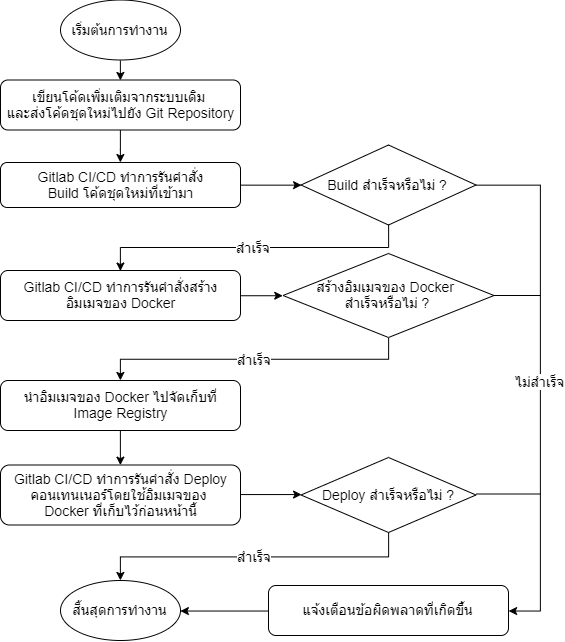
\includegraphics[width=1\textwidth]{gitlab-flow.png}  
	\caption{แผนผังวิธีการ Deploy โค้ดชุดใหม่ของเซอร์วิส Ad Report}
	\label{Fig:adreport-diagram}
\end{figure}
    \chapter{ผลการปฏิบัติงาน}
\label{chapter:result จากการปฏิบัติงานสหกิจศึกษาที่ บริษัท วงใน มีเดีย จำกัด (สำนักงานใหญ่) ด้วยตำแหน่ง Software Engineer (Backend) เป็นระยะเวลา 6 เดือน ตั้ง 4 มิถุนายน พ.ศ.2562 จนถึง 29 พฤศจิกายน พ.ศ.2562 สามารถสรุปผลการปฏิบัติงานได้ดังนี้
	
\section{ผลการปฏิบัติงาน}
ฟังก์ชันหลักของระบบจัดการโฆษณาแบบจำกัดจำนวนการคลิกและการแสดงโฆษณา สามารถทำงานตามที่ออกแบบไว้ โดยสามารถจำกัดการแสดงผลโฆษณาด้วยจำนวนการคลิกของโฆษณา และสามารถสร้างอีเมลรายงานสถิติของโฆษณาตามที่ UX/UI ของ Squad เป็นผู้ออกแบบ ส่งไปยังลูกค้าได้โดยอัตโนมัติได้ นอกจากนี้ก็จะมีหน้าแอดมินสำหรับให้เจ้าหน้าที่ที่เกี่ยวข้องเข้ามาใช้งานเซอร์วิส Ad Report ได้ โดยจะมีฟังก์ชันต่าง ๆ ดังนี
\begin{itemize}
	\item แก้ไขข้อมูลต่าง ๆ ของร้านได้โดยการกดไปที่ไอคอนดินสอสีฟ้า
	\item ส่งอีเมลรายงานสถิติของโฆษณารายสัปดาห์โดยการกดไปที่ปุ่ม ACTIONS สีแดง (สำหรับใช้งานในกรณีที่การส่งอัตโนมัติเกิดข้อผิดพลาด เจ้าหน้าที่คนอื่นจะสามารถส่งอีเมลรายงานด้วยตนเองได้) 
\end{itemize}

สำหรับหน้าแอดมินนั้น ได้ใช้เฟรมเวิร์คที่จัดเตรียมไว้ให้อยู่แล้ว ซึ่งพัฒนาโดยทีม Software Engineer (Frontend) ของบริษัท ใช้ React ซึ่งเป็น ไลบรารีสำหรับสร้าง User Interface ของเว็บไซต์ด้วยภาษา Javascript ~\cite{react} และภายในรายงานสถิติของโฆษณาที่ส่งไปยังอีเมลของลูกค้าจะประกอบไปด้วยข้อมูลต่าง ๆ ได้แก่
\begin{itemize}
	\item ชื่อร้าน
	\item ช่วงเวลาของรายงาน
	\item จำนวนครั้งที่แสดงผลโฆษณาในช่วงเวลาของรายงาน
	\item จำนวนครั้งที่มีผู้ใช้คลิกเข้าไปที่โฆษณาในช่วงเวลาของรายงาน
	\item แผนภูมิแสดงจำนวนครั้งที่แสดงผลโฆษณาในช่วงเวลาของรายงานต่อวัน
	\item แผนภูมิแสดงจำนวนครั้งที่มีผู้ใช้คลิกเข้าไปที่โฆษณาในช่วงเวลาของรายงานต่อวัน
	\item จำนวนคลิกของโฆษณาที่ใช้ไปแล้ว
	\item จำนวนคลิกของโฆษณาคงเหลือ
\end{itemize}

\begin{figure}[!h]
	\centering
	\subfigure[]{
		\label{Fig:adminui:list}
		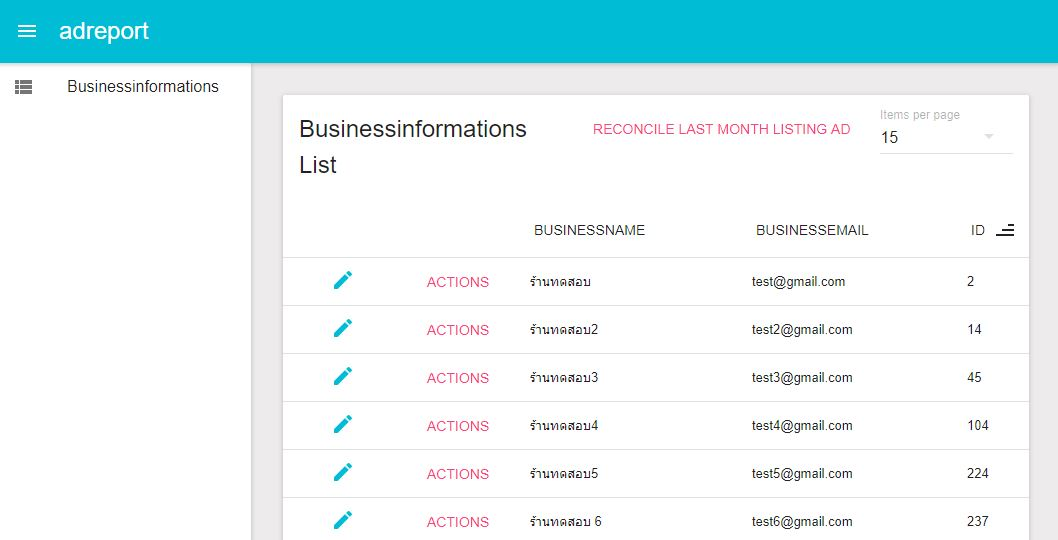
\includegraphics[width=0.9\textwidth]{admin-ui-1}  
	}
	\subfigure[]{
		\label{Fig:adminui:edit}
		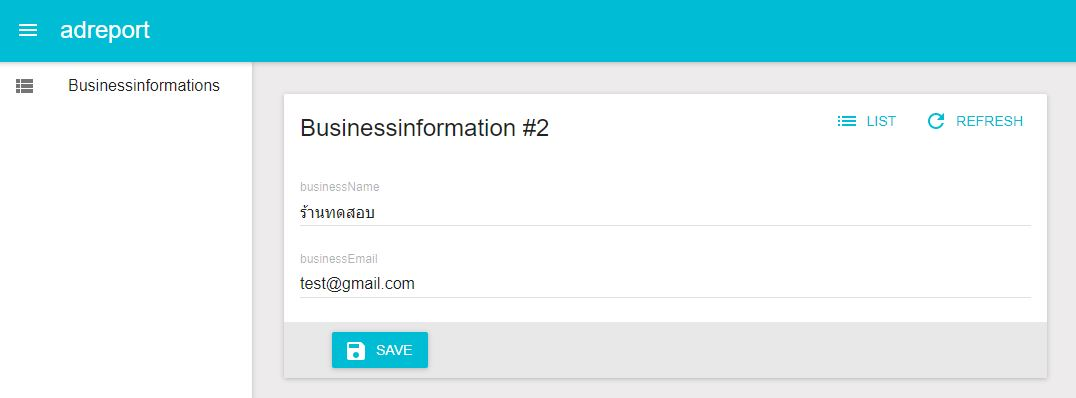
\includegraphics[width=0.9\textwidth]{admin-ui-2}  
	}
	\caption{หน้าแอดมินสำหรับให้เจ้าหน้าที่ที่เกี่ยวข้องเข้ามาใช้งานเซอร์วิส Ad Report (ก) และหน้าแก้ไขข้อมูลต่าง ๆ ของร้าน (ข)}
	\label{Fig:adminui}
\end{figure}

\begin{figure}[!h]
	\centering
	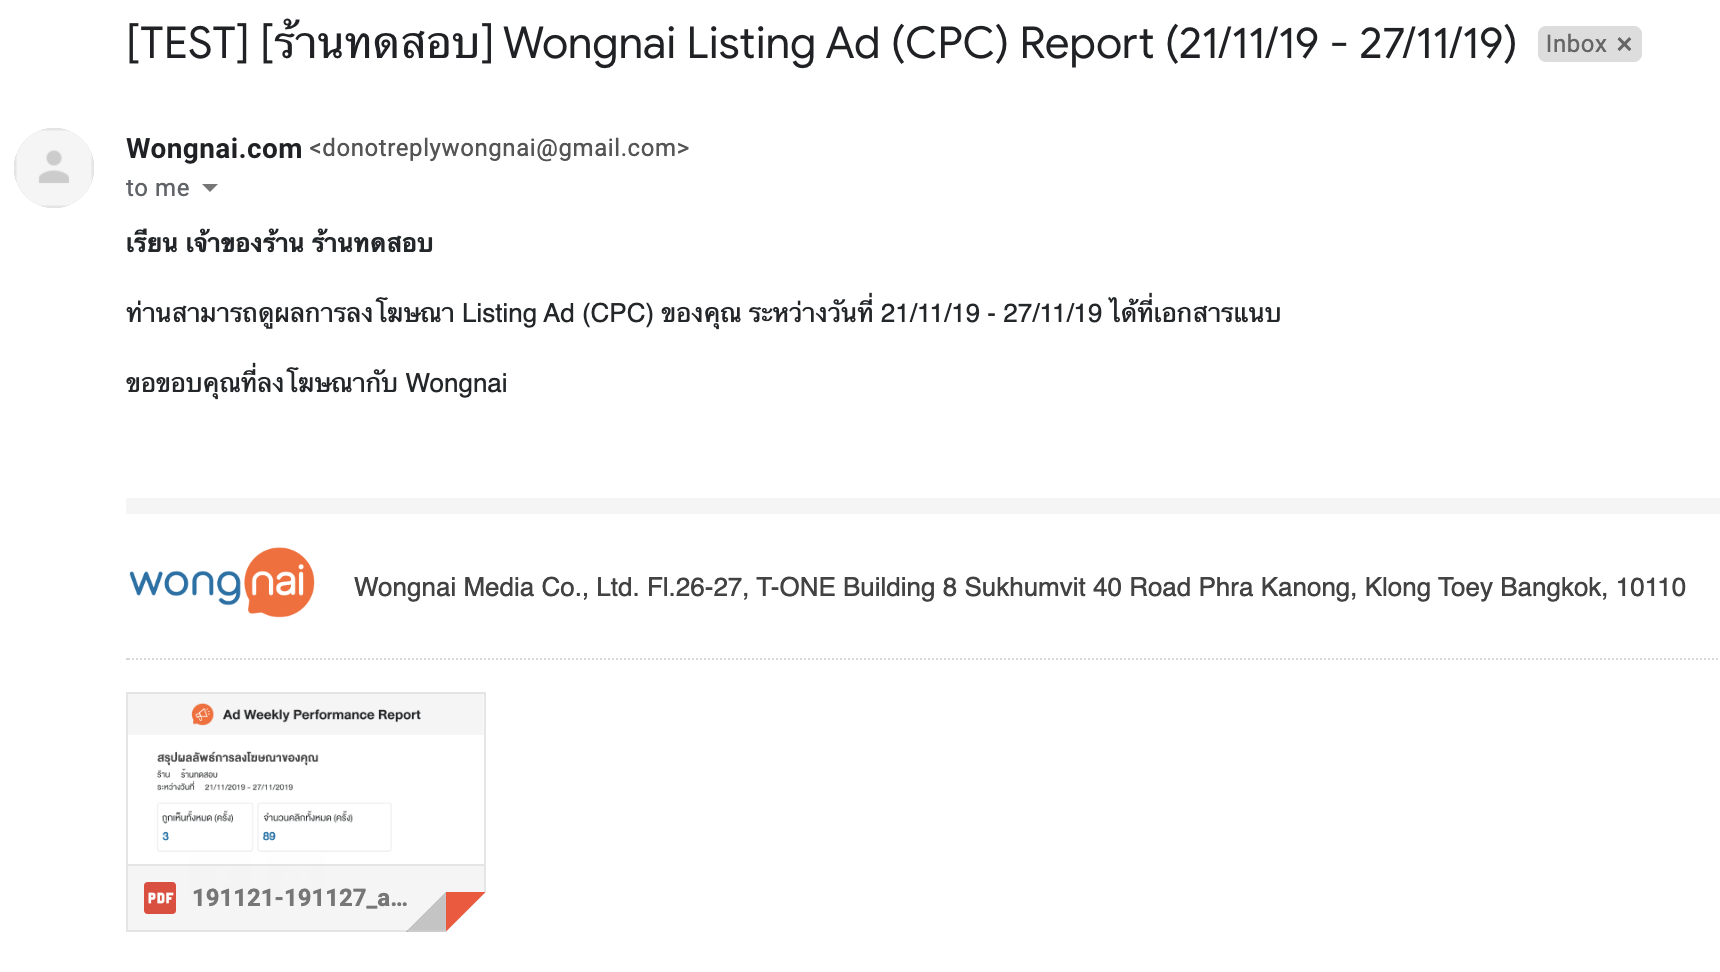
\includegraphics[width=0.875\textwidth]{report-email.png}  
	\caption{อีเมลรายงานสถิติของโฆษณาที่ส่งให้ลูกค้า}
	\label{Fig:report-email}
\end{figure}

\begin{figure}[!p]
	\centering
	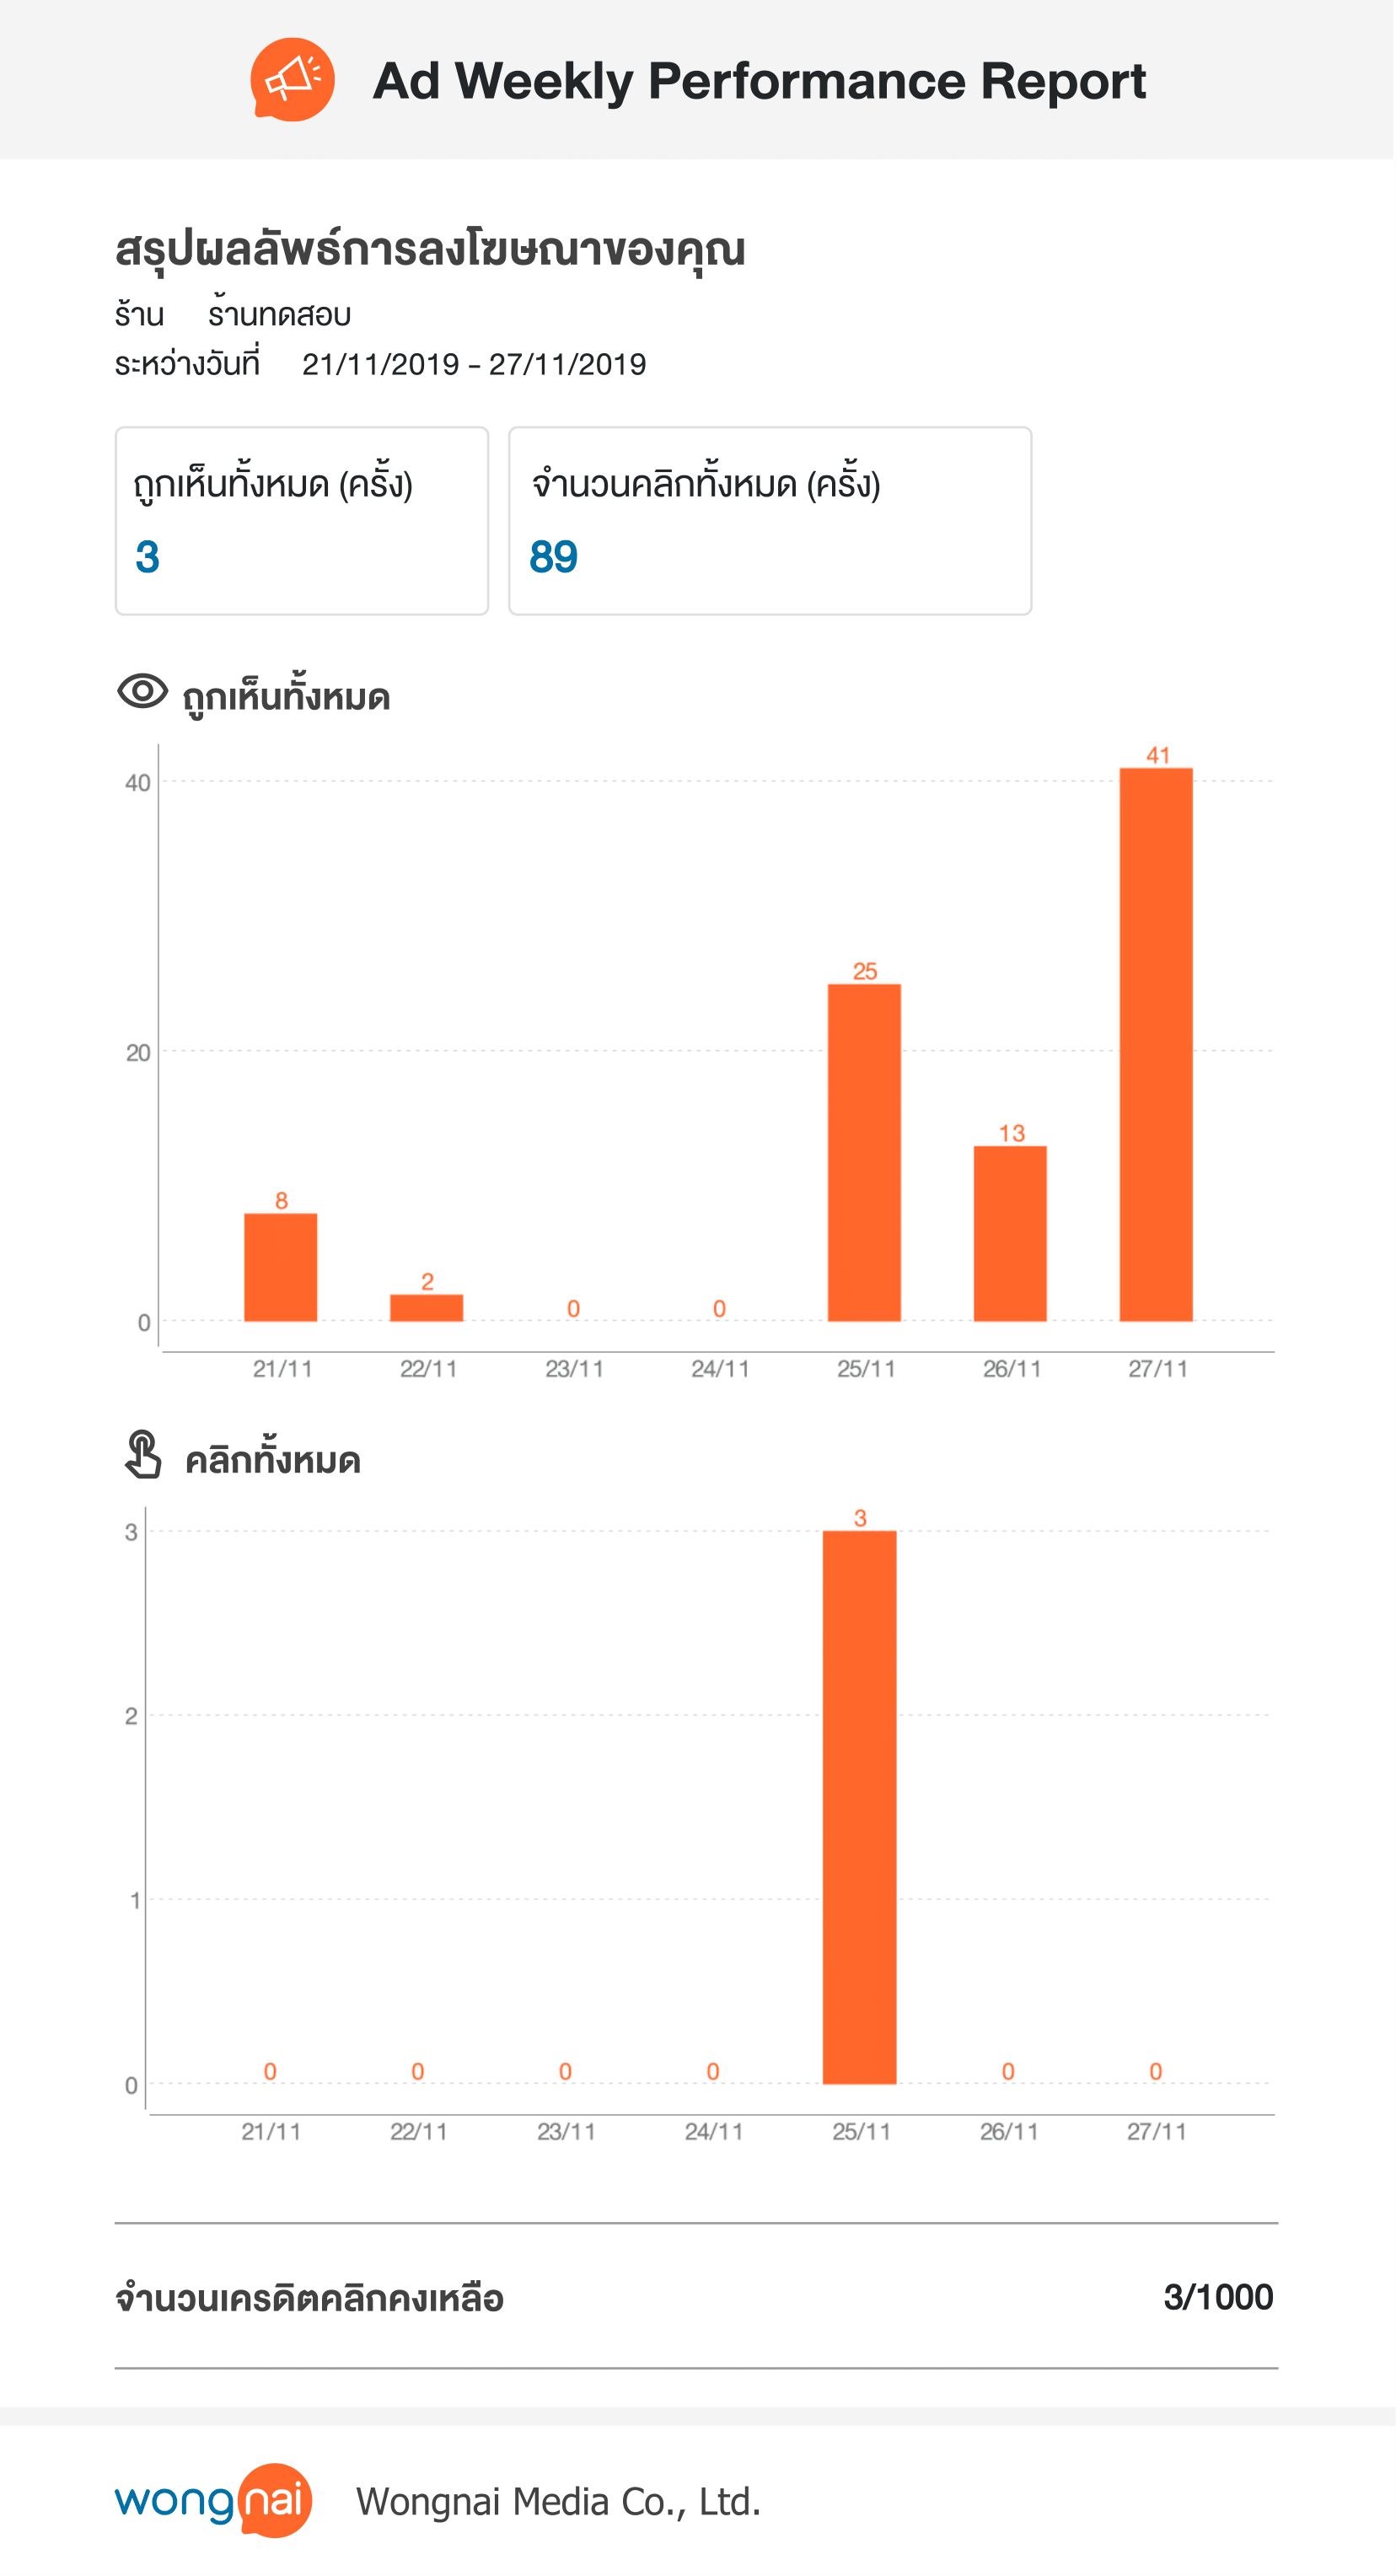
\includegraphics[width=0.9\textwidth]{report.png}  
	\caption{รายงานสถิติของโฆษณาที่ส่งให้ลูกค้า}
	\label{Fig:report}
\end{figure}

    
    \clearpage
    \addcontentsline{toc}{chapter}{บรรณานุกรม}
    \bibliographystyle{IEEEtran}
    \bibliography{reference}
    
    \startappendix
    \chapter{เรื่องที่หนึ่ง}
    
\end{document}